\documentclass[1p]{elsarticle_modified}
%\bibliographystyle{elsarticle-num}

%\usepackage[colorlinks]{hyperref}
%\usepackage{abbrmath_seonhwa} %\Abb, \Ascr, \Acal ,\Abf, \Afrak
\usepackage{amsfonts}
\usepackage{amssymb}
\usepackage{amsmath}
\usepackage{amsthm}
\usepackage{scalefnt}
\usepackage{amsbsy}
\usepackage{kotex}
\usepackage{caption}
\usepackage{subfig}
\usepackage{color}
\usepackage{graphicx}
\usepackage{xcolor} %% white, black, red, green, blue, cyan, magenta, yellow
\usepackage{float}
\usepackage{setspace}
\usepackage{hyperref}

\usepackage{tikz}
\usetikzlibrary{arrows}

\usepackage{multirow}
\usepackage{array} % fixed length table
\usepackage{hhline}

%%%%%%%%%%%%%%%%%%%%%
\makeatletter
\renewcommand*\env@matrix[1][\arraystretch]{%
	\edef\arraystretch{#1}%
	\hskip -\arraycolsep
	\let\@ifnextchar\new@ifnextchar
	\array{*\c@MaxMatrixCols c}}
\makeatother %https://tex.stackexchange.com/questions/14071/how-can-i-increase-the-line-spacing-in-a-matrix
%%%%%%%%%%%%%%%

\usepackage[normalem]{ulem}

\newcommand{\msout}[1]{\ifmmode\text{\sout{\ensuremath{#1}}}\else\sout{#1}\fi}
%SOURCE: \msout is \stkout macro in https://tex.stackexchange.com/questions/20609/strikeout-in-math-mode

\newcommand{\cancel}[1]{
	\ifmmode
	{\color{red}\msout{#1}}
	\else
	{\color{red}\sout{#1}}
	\fi
}

\newcommand{\add}[1]{
	{\color{blue}\uwave{#1}}
}

\newcommand{\replace}[2]{
	\ifmmode
	{\color{red}\msout{#1}}{\color{blue}\uwave{#2}}
	\else
	{\color{red}\sout{#1}}{\color{blue}\uwave{#2}}
	\fi
}

\newcommand{\Sol}{\mathcal{S}} %segment
\newcommand{\D}{D} %diagram
\newcommand{\A}{\mathcal{A}} %arc


%%%%%%%%%%%%%%%%%%%%%%%%%%%%%5 test

\def\sl{\operatorname{\textup{SL}}(2,\Cbb)}
\def\psl{\operatorname{\textup{PSL}}(2,\Cbb)}
\def\quan{\mkern 1mu \triangleright \mkern 1mu}

\theoremstyle{definition}
\newtheorem{thm}{Theorem}[section]
\newtheorem{prop}[thm]{Proposition}
\newtheorem{lem}[thm]{Lemma}
\newtheorem{ques}[thm]{Question}
\newtheorem{cor}[thm]{Corollary}
\newtheorem{defn}[thm]{Definition}
\newtheorem{exam}[thm]{Example}
\newtheorem{rmk}[thm]{Remark}
\newtheorem{alg}[thm]{Algorithm}

\newcommand{\I}{\sqrt{-1}}
\begin{document}

%\begin{frontmatter}
%
%\title{Boundary parabolic representations of knots up to 8 crossings}
%
%%% Group authors per affiliation:
%\author{Yunhi Cho} 
%\address{Department of Mathematics, University of Seoul, Seoul, Korea}
%\ead{yhcho@uos.ac.kr}
%
%
%\author{Seonhwa Kim} %\fnref{s_kim}}
%\address{Center for Geometry and Physics, Institute for Basic Science, Pohang, 37673, Korea}
%\ead{ryeona17@ibs.re.kr}
%
%\author{Hyuk Kim}
%\address{Department of Mathematical Sciences, Seoul National University, Seoul 08826, Korea}
%\ead{hyukkim@snu.ac.kr}
%
%\author{Seokbeom Yoon}
%\address{Department of Mathematical Sciences, Seoul National University, Seoul, 08826,  Korea}
%\ead{sbyoon15@snu.ac.kr}
%
%\begin{abstract}
%We find all boundary parabolic representation of knots up to 8 crossings.
%
%\end{abstract}
%\begin{keyword}
%    \MSC[2010] 57M25 
%\end{keyword}
%
%\end{frontmatter}

%\linenumbers
%\tableofcontents
%
\newcommand\colored[1]{\textcolor{white}{\rule[-0.35ex]{0.8em}{1.4ex}}\kern-0.8em\color{red} #1}%
%\newcommand\colored[1]{\textcolor{white}{ #1}\kern-2.17ex	\textcolor{white}{ #1}\kern-1.81ex	\textcolor{white}{ #1}\kern-2.15ex\color{red}#1	}

{\Large $\underline{12a_{0913}~(K12a_{0913})}$}

\setlength{\tabcolsep}{10pt}
\renewcommand{\arraystretch}{1.6}
\vspace{1cm}\begin{tabular}{m{100pt}>{\centering\arraybackslash}m{274pt}}
\multirow{5}{120pt}{
	\centering
	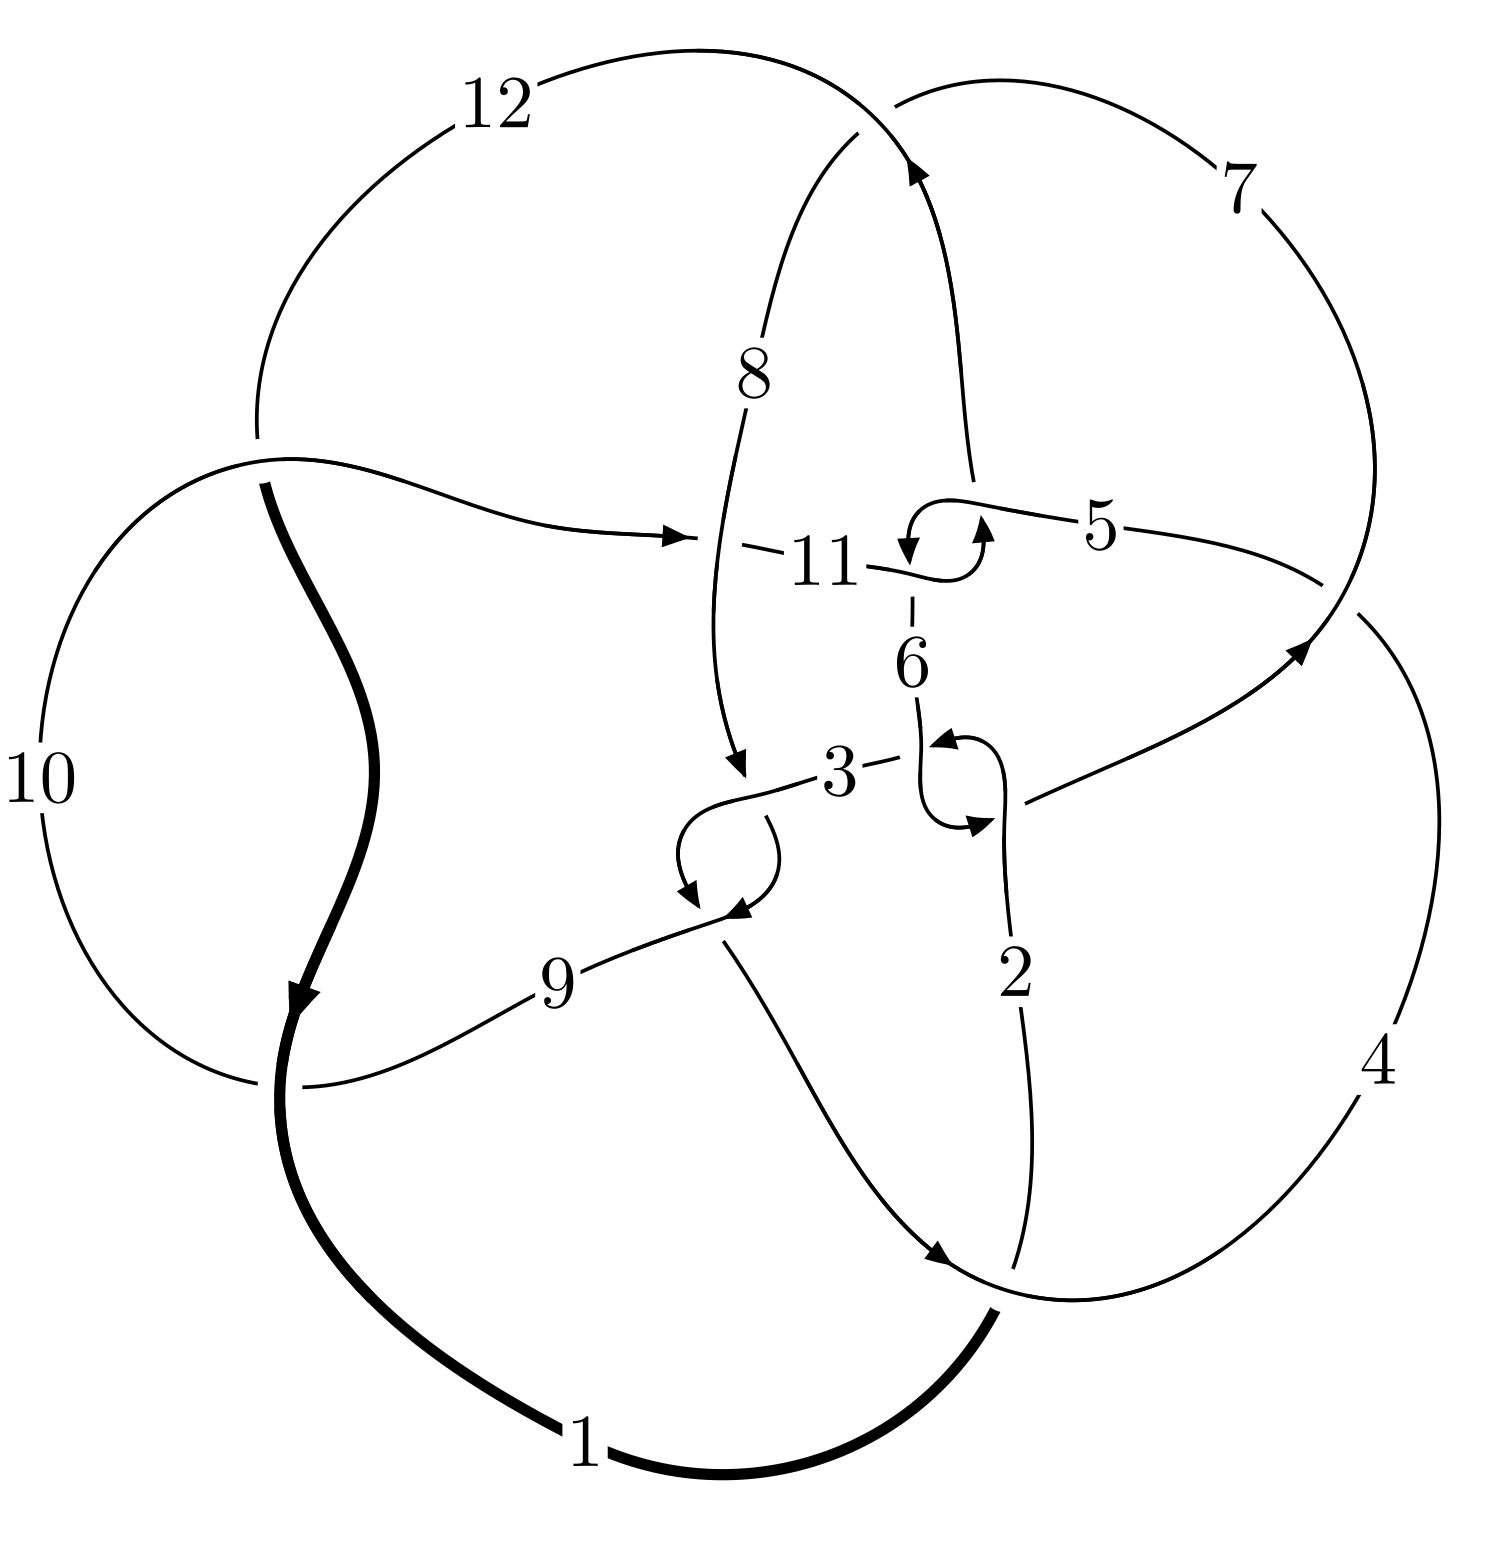
\includegraphics[width=112pt]{../../../GIT/diagram.site/Diagrams/png/1714_12a_0913.png}\\
\ \ \ A knot diagram\footnotemark}&
\allowdisplaybreaks
\textbf{Linearized knot diagam} \\
\cline{2-2}
 &
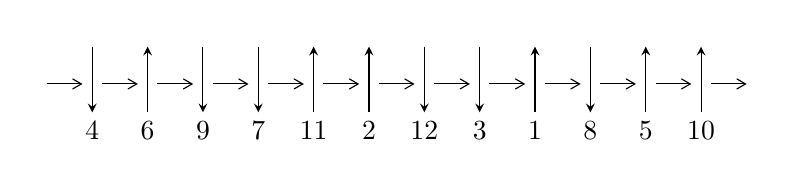
\begin{tikzpicture}[x=20pt, y=17pt]
	% nodes
	\node (C0) at (0, 0) {};
	\node (C1) at (1, 0) {};
	\node (C1U) at (1, +1) {};
	\node (C1D) at (1, -1) {4};

	\node (C2) at (2, 0) {};
	\node (C2U) at (2, +1) {};
	\node (C2D) at (2, -1) {6};

	\node (C3) at (3, 0) {};
	\node (C3U) at (3, +1) {};
	\node (C3D) at (3, -1) {9};

	\node (C4) at (4, 0) {};
	\node (C4U) at (4, +1) {};
	\node (C4D) at (4, -1) {7};

	\node (C5) at (5, 0) {};
	\node (C5U) at (5, +1) {};
	\node (C5D) at (5, -1) {11};

	\node (C6) at (6, 0) {};
	\node (C6U) at (6, +1) {};
	\node (C6D) at (6, -1) {2};

	\node (C7) at (7, 0) {};
	\node (C7U) at (7, +1) {};
	\node (C7D) at (7, -1) {12};

	\node (C8) at (8, 0) {};
	\node (C8U) at (8, +1) {};
	\node (C8D) at (8, -1) {3};

	\node (C9) at (9, 0) {};
	\node (C9U) at (9, +1) {};
	\node (C9D) at (9, -1) {1};

	\node (C10) at (10, 0) {};
	\node (C10U) at (10, +1) {};
	\node (C10D) at (10, -1) {8};

	\node (C11) at (11, 0) {};
	\node (C11U) at (11, +1) {};
	\node (C11D) at (11, -1) {5};

	\node (C12) at (12, 0) {};
	\node (C12U) at (12, +1) {};
	\node (C12D) at (12, -1) {10};
	\node (C13) at (13, 0) {};

	% arrows
	\draw[->,>={angle 60}]
	(C0) edge (C1) (C1) edge (C2) (C2) edge (C3) (C3) edge (C4) (C4) edge (C5) (C5) edge (C6) (C6) edge (C7) (C7) edge (C8) (C8) edge (C9) (C9) edge (C10) (C10) edge (C11) (C11) edge (C12) (C12) edge (C13) ;	\draw[->,>=stealth]
	(C1U) edge (C1D) (C2D) edge (C2U) (C3U) edge (C3D) (C4U) edge (C4D) (C5D) edge (C5U) (C6D) edge (C6U) (C7U) edge (C7D) (C8U) edge (C8D) (C9D) edge (C9U) (C10U) edge (C10D) (C11D) edge (C11U) (C12D) edge (C12U) ;
	\end{tikzpicture} \\
\hhline{~~} \\& 
\textbf{Solving Sequence} \\ \cline{2-2} 
 &
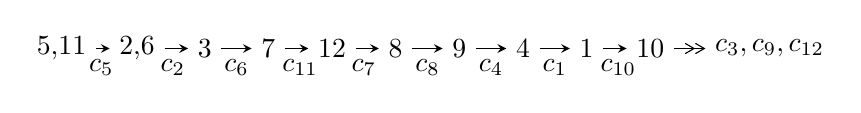
\begin{tikzpicture}[x=23pt, y=7pt]
	% node
	\node (A0) at (-1/8, 0) {5,11};
	\node (A1) at (17/16, 0) {2,6};
	\node (A2) at (17/8, 0) {3};
	\node (A3) at (25/8, 0) {7};
	\node (A4) at (33/8, 0) {12};
	\node (A5) at (41/8, 0) {8};
	\node (A6) at (49/8, 0) {9};
	\node (A7) at (57/8, 0) {4};
	\node (A8) at (65/8, 0) {1};
	\node (A9) at (73/8, 0) {10};
	\node (C1) at (1/2, -1) {$c_{5}$};
	\node (C2) at (13/8, -1) {$c_{2}$};
	\node (C3) at (21/8, -1) {$c_{6}$};
	\node (C4) at (29/8, -1) {$c_{11}$};
	\node (C5) at (37/8, -1) {$c_{7}$};
	\node (C6) at (45/8, -1) {$c_{8}$};
	\node (C7) at (53/8, -1) {$c_{4}$};
	\node (C8) at (61/8, -1) {$c_{1}$};
	\node (C9) at (69/8, -1) {$c_{10}$};
	\node (A10) at (11, 0) {$c_{3},c_{9},c_{12}$};

	% edge
	\draw[->,>=stealth]	
	(A0) edge (A1) (A1) edge (A2) (A2) edge (A3) (A3) edge (A4) (A4) edge (A5) (A5) edge (A6) (A6) edge (A7) (A7) edge (A8) (A8) edge (A9) ;
	\draw[->>,>={angle 60}]	
	(A9) edge (A10);
\end{tikzpicture} \\ 

\end{tabular} \\

\footnotetext{
The image of knot diagram is generated by the software ``\textbf{Draw programme}" developed by Andrew Bartholomew(\url{http://www.layer8.co.uk/maths/draw/index.htm\#Running-draw}), where we modified some parts for our purpose(\url{https://github.com/CATsTAILs/LinksPainter}).
}\phantom \\ \newline 
\centering \textbf{Ideals for irreducible components\footnotemark of $X_{\text{par}}$} 
 
\begin{align*}
I^u_{1}&=\langle 
-1.23675\times10^{864} u^{158}+8.56639\times10^{864} u^{157}+\cdots+1.08073\times10^{866} b-2.39792\times10^{869},\\
\phantom{I^u_{1}}&\phantom{= \langle  }9.55810\times10^{868} u^{158}+2.76471\times10^{869} u^{157}+\cdots+6.48654\times10^{869} a-4.53046\times10^{873},\\
\phantom{I^u_{1}}&\phantom{= \langle  }u^{159}+u^{158}+\cdots-95441 u-24008\rangle \\
I^u_{2}&=\langle 
-7.72164\times10^{68} u^{49}-3.42499\times10^{69} u^{48}+\cdots+1.57649\times10^{69} b+6.72123\times10^{70},\\
\phantom{I^u_{2}}&\phantom{= \langle  }5.04081\times10^{69} u^{49}-1.88268\times10^{70} u^{48}+\cdots+4.72946\times10^{69} a+3.67110\times10^{71},\;u^{50}+11 u^{48}+\cdots+15 u-9\rangle \\
\\
\end{align*}
\raggedright * 2 irreducible components of $\dim_{\mathbb{C}}=0$, with total 209 representations.\\
\footnotetext{All coefficients of polynomials are rational numbers. But the coefficients are sometimes approximated in decimal forms when there is not enough margin.}
\newpage
\renewcommand{\arraystretch}{1}
\centering \section*{I. $I^u_{1}= \langle -1.24\times10^{864} u^{158}+8.57\times10^{864} u^{157}+\cdots+1.08\times10^{866} b-2.40\times10^{869},\;9.56\times10^{868} u^{158}+2.76\times10^{869} u^{157}+\cdots+6.49\times10^{869} a-4.53\times10^{873},\;u^{159}+u^{158}+\cdots-95441 u-24008 \rangle$}
\flushleft \textbf{(i) Arc colorings}\\
\begin{tabular}{m{7pt} m{180pt} m{7pt} m{180pt} }
\flushright $a_{5}=$&$\begin{pmatrix}1\\0\end{pmatrix}$ \\
\flushright $a_{11}=$&$\begin{pmatrix}0\\u\end{pmatrix}$ \\
\flushright $a_{2}=$&$\begin{pmatrix}-0.147353 u^{158}-0.426224 u^{157}+\cdots+31421.1 u+6984.41\\0.0114437 u^{158}-0.0792649 u^{157}+\cdots+8457.34 u+2218.80\end{pmatrix}$ \\
\flushright $a_{6}=$&$\begin{pmatrix}1\\- u^2\end{pmatrix}$ \\
\flushright $a_{3}=$&$\begin{pmatrix}0.00578855 u^{158}-0.0950449 u^{157}+\cdots+9725.12 u+2508.09\\0.156936 u^{158}+0.237303 u^{157}+\cdots-12211.3 u-2055.51\end{pmatrix}$ \\
\flushright $a_{7}=$&$\begin{pmatrix}0.357898 u^{158}+0.241453 u^{157}+\cdots+2030.58 u+2910.40\\-0.0884457 u^{158}-0.131877 u^{157}+\cdots+7349.06 u+1277.73\end{pmatrix}$ \\
\flushright $a_{12}=$&$\begin{pmatrix}u\\u\end{pmatrix}$ \\
\flushright $a_{8}=$&$\begin{pmatrix}-0.0431647 u^{158}-0.0826383 u^{157}+\cdots+5777.86 u+1157.47\\-0.489509 u^{158}-0.455968 u^{157}+\cdots+11096.3 u-475.196\end{pmatrix}$ \\
\flushright $a_{9}=$&$\begin{pmatrix}-0.00256598 u^{158}+0.0441083 u^{157}+\cdots-4552.86 u-1152.68\\-0.0179626 u^{158}+0.0140324 u^{157}+\cdots-2580.84 u-742.756\end{pmatrix}$ \\
\flushright $a_{4}=$&$\begin{pmatrix}-0.126198 u^{158}-0.401253 u^{157}+\cdots+31148.5 u+7083.44\\0.0725043 u^{158}+0.0139851 u^{157}+\cdots+3714.98 u+1451.08\end{pmatrix}$ \\
\flushright $a_{1}=$&$\begin{pmatrix}0.0722265 u^{158}-0.00605847 u^{157}+\cdots+5929.89 u+1975.45\\0.0504978 u^{158}-0.0108585 u^{157}+\cdots+5189.42 u+1635.88\end{pmatrix}$ \\
\flushright $a_{10}=$&$\begin{pmatrix}0.0756881 u^{158}+0.122223 u^{157}+\cdots-7580.53 u-1432.70\\0.0634567 u^{158}+0.0797254 u^{157}+\cdots-4471.11 u-724.940\end{pmatrix}$\\&\end{tabular}
\flushleft \textbf{(ii) Obstruction class $= -1$}\\~\\
\flushleft \textbf{(iii) Cusp Shapes $= -2.37885 u^{158}+1.78647 u^{157}+\cdots-358356. u-105900.$}\\~\\
\newpage\renewcommand{\arraystretch}{1}
\flushleft \textbf{(iv) u-Polynomials at the component}\newline \\
\begin{tabular}{m{50pt}|m{274pt}}
Crossings & \hspace{64pt}u-Polynomials at each crossing \\
\hline $$\begin{aligned}c_{1}\end{aligned}$$&$\begin{aligned}
&u^{159}-8 u^{158}+\cdots+80215197 u-1927186
\end{aligned}$\\
\hline $$\begin{aligned}c_{2},c_{6}\end{aligned}$$&$\begin{aligned}
&u^{159}-3 u^{158}+\cdots-3046266 u-178861
\end{aligned}$\\
\hline $$\begin{aligned}c_{3},c_{8}\end{aligned}$$&$\begin{aligned}
&u^{159}- u^{158}+\cdots-8744042 u+1097059
\end{aligned}$\\
\hline $$\begin{aligned}c_{4}\end{aligned}$$&$\begin{aligned}
&u^{159}-7 u^{158}+\cdots+32390037 u-6440257
\end{aligned}$\\
\hline $$\begin{aligned}c_{5},c_{11}\end{aligned}$$&$\begin{aligned}
&u^{159}+u^{158}+\cdots-95441 u-24008
\end{aligned}$\\
\hline $$\begin{aligned}c_{7}\end{aligned}$$&$\begin{aligned}
&u^{159}+15 u^{158}+\cdots+43507681 u-2774953
\end{aligned}$\\
\hline $$\begin{aligned}c_{9},c_{12}\end{aligned}$$&$\begin{aligned}
&u^{159}+5 u^{158}+\cdots+159249 u+8893
\end{aligned}$\\
\hline $$\begin{aligned}c_{10}\end{aligned}$$&$\begin{aligned}
&u^{159}-15 u^{158}+\cdots-333964577 u+95115071
\end{aligned}$\\
\hline
\end{tabular}\\~\\
\newpage\renewcommand{\arraystretch}{1}
\flushleft \textbf{(v) Riley Polynomials at the component}\newline \\
\begin{tabular}{m{50pt}|m{274pt}}
Crossings & \hspace{64pt}Riley Polynomials at each crossing \\
\hline $$\begin{aligned}c_{1}\end{aligned}$$&$\begin{aligned}
&y^{159}-82 y^{158}+\cdots+3262006438404145 y-3714045878596
\end{aligned}$\\
\hline $$\begin{aligned}c_{2},c_{6}\end{aligned}$$&$\begin{aligned}
&y^{159}+115 y^{158}+\cdots+126566005786 y-31991257321
\end{aligned}$\\
\hline $$\begin{aligned}c_{3},c_{8}\end{aligned}$$&$\begin{aligned}
&y^{159}-105 y^{158}+\cdots+42991384255528 y-1203538449481
\end{aligned}$\\
\hline $$\begin{aligned}c_{4}\end{aligned}$$&$\begin{aligned}
&y^{159}-61 y^{158}+\cdots+774738334454811 y-41476910226049
\end{aligned}$\\
\hline $$\begin{aligned}c_{5},c_{11}\end{aligned}$$&$\begin{aligned}
&y^{159}+97 y^{158}+\cdots-15736846703 y-576384064
\end{aligned}$\\
\hline $$\begin{aligned}c_{7}\end{aligned}$$&$\begin{aligned}
&y^{159}-57 y^{158}+\cdots+1120931842505265 y-7700364152209
\end{aligned}$\\
\hline $$\begin{aligned}c_{9},c_{12}\end{aligned}$$&$\begin{aligned}
&y^{159}+127 y^{158}+\cdots+291286079 y-79085449
\end{aligned}$\\
\hline $$\begin{aligned}c_{10}\end{aligned}$$&$\begin{aligned}
&y^{159}-59 y^{158}+\cdots+1754195507846337117 y-9046876731335041
\end{aligned}$\\
\hline
\end{tabular}\\~\\
\newpage\flushleft \textbf{(vi) Complex Volumes and Cusp Shapes}
$$\begin{array}{c|c|c}  
\text{Solutions to }I^u_{1}& \I (\text{vol} + \sqrt{-1}CS) & \text{Cusp shape}\\
 \hline 
\begin{aligned}
u &= \phantom{-}0.331449 + 0.959871 I \\
a &= -1.87562 - 0.22966 I \\
b &= -2.02429 - 0.05797 I\end{aligned}
 & -9.26485 + 9.17013 I & \phantom{-0.000000 } 0 \\ \hline\begin{aligned}
u &= \phantom{-}0.331449 - 0.959871 I \\
a &= -1.87562 + 0.22966 I \\
b &= -2.02429 + 0.05797 I\end{aligned}
 & -9.26485 - 9.17013 I & \phantom{-0.000000 } 0 \\ \hline\begin{aligned}
u &= -1.014430 + 0.098634 I \\
a &= \phantom{-}0.451232 - 0.570464 I \\
b &= \phantom{-}0.04601 + 1.78543 I\end{aligned}
 & -0.82025 + 3.44925 I & \phantom{-0.000000 } 0 \\ \hline\begin{aligned}
u &= -1.014430 - 0.098634 I \\
a &= \phantom{-}0.451232 + 0.570464 I \\
b &= \phantom{-}0.04601 - 1.78543 I\end{aligned}
 & -0.82025 - 3.44925 I & \phantom{-0.000000 } 0 \\ \hline\begin{aligned}
u &= -0.105746 + 1.013950 I \\
a &= -0.38849 - 3.37577 I \\
b &= \phantom{-}0.19676 - 2.47170 I\end{aligned}
 & -1.18179 - 3.20636 I & \phantom{-0.000000 } 0 \\ \hline\begin{aligned}
u &= -0.105746 - 1.013950 I \\
a &= -0.38849 + 3.37577 I \\
b &= \phantom{-}0.19676 + 2.47170 I\end{aligned}
 & -1.18179 + 3.20636 I & \phantom{-0.000000 } 0 \\ \hline\begin{aligned}
u &= \phantom{-}1.027040 + 0.093678 I \\
a &= \phantom{-}0.325147 + 0.603162 I \\
b &= \phantom{-}0.14935 - 1.94748 I\end{aligned}
 & -5.64108 - 7.19608 I & \phantom{-0.000000 } 0 \\ \hline\begin{aligned}
u &= \phantom{-}1.027040 - 0.093678 I \\
a &= \phantom{-}0.325147 - 0.603162 I \\
b &= \phantom{-}0.14935 + 1.94748 I\end{aligned}
 & -5.64108 + 7.19608 I & \phantom{-0.000000 } 0 \\ \hline\begin{aligned}
u &= -0.007128 + 0.966467 I \\
a &= -0.91257 - 3.00884 I \\
b &= \phantom{-}0.265736 - 0.196627 I\end{aligned}
 & -5.35993 - 0.16362 I & \phantom{-0.000000 } 0 \\ \hline\begin{aligned}
u &= -0.007128 - 0.966467 I \\
a &= -0.91257 + 3.00884 I \\
b &= \phantom{-}0.265736 + 0.196627 I\end{aligned}
 & -5.35993 + 0.16362 I & \phantom{-0.000000 } 0\\
 \hline 
 \end{array}$$\newpage$$\begin{array}{c|c|c}  
\text{Solutions to }I^u_{1}& \I (\text{vol} + \sqrt{-1}CS) & \text{Cusp shape}\\
 \hline 
\begin{aligned}
u &= -0.206168 + 1.014050 I \\
a &= \phantom{-}0.702066 + 0.183119 I \\
b &= -0.707965 + 0.099887 I\end{aligned}
 & -4.72393 + 1.17967 I & \phantom{-0.000000 } 0 \\ \hline\begin{aligned}
u &= -0.206168 - 1.014050 I \\
a &= \phantom{-}0.702066 - 0.183119 I \\
b &= -0.707965 - 0.099887 I\end{aligned}
 & -4.72393 - 1.17967 I & \phantom{-0.000000 } 0 \\ \hline\begin{aligned}
u &= \phantom{-}0.963567 + 0.007515 I \\
a &= \phantom{-}0.347493 - 0.236451 I \\
b &= \phantom{-}0.241095 + 1.028930 I\end{aligned}
 & -3.13062 - 0.11256 I & \phantom{-0.000000 } 0 \\ \hline\begin{aligned}
u &= \phantom{-}0.963567 - 0.007515 I \\
a &= \phantom{-}0.347493 + 0.236451 I \\
b &= \phantom{-}0.241095 - 1.028930 I\end{aligned}
 & -3.13062 + 0.11256 I & \phantom{-0.000000 } 0 \\ \hline\begin{aligned}
u &= \phantom{-}0.027589 + 1.039060 I \\
a &= \phantom{-}0.43849 + 2.47650 I \\
b &= \phantom{-}0.71163 + 1.31819 I\end{aligned}
 & -3.47849 + 0.04457 I & \phantom{-0.000000 } 0 \\ \hline\begin{aligned}
u &= \phantom{-}0.027589 - 1.039060 I \\
a &= \phantom{-}0.43849 - 2.47650 I \\
b &= \phantom{-}0.71163 - 1.31819 I\end{aligned}
 & -3.47849 - 0.04457 I & \phantom{-0.000000 } 0 \\ \hline\begin{aligned}
u &= \phantom{-}0.005856 + 0.947362 I \\
a &= \phantom{-}1.47155 + 1.25478 I \\
b &= \phantom{-}1.71025 + 0.16199 I\end{aligned}
 & -3.13181 + 0.06061 I & \phantom{-0.000000 } 0 \\ \hline\begin{aligned}
u &= \phantom{-}0.005856 - 0.947362 I \\
a &= \phantom{-}1.47155 - 1.25478 I \\
b &= \phantom{-}1.71025 - 0.16199 I\end{aligned}
 & -3.13181 - 0.06061 I & \phantom{-0.000000 } 0 \\ \hline\begin{aligned}
u &= -0.047301 + 1.053540 I \\
a &= -0.846698 + 0.406491 I \\
b &= \phantom{-}0.278061 - 0.181203 I\end{aligned}
 & -3.89278 - 1.46765 I & \phantom{-0.000000 } 0 \\ \hline\begin{aligned}
u &= -0.047301 - 1.053540 I \\
a &= -0.846698 - 0.406491 I \\
b &= \phantom{-}0.278061 + 0.181203 I\end{aligned}
 & -3.89278 + 1.46765 I & \phantom{-0.000000 } 0\\
 \hline 
 \end{array}$$\newpage$$\begin{array}{c|c|c}  
\text{Solutions to }I^u_{1}& \I (\text{vol} + \sqrt{-1}CS) & \text{Cusp shape}\\
 \hline 
\begin{aligned}
u &= -0.796936 + 0.498050 I \\
a &= -0.378245 + 0.302345 I \\
b &= -0.064321 + 0.714699 I\end{aligned}
 & -2.37488 + 1.85883 I & \phantom{-0.000000 } 0 \\ \hline\begin{aligned}
u &= -0.796936 - 0.498050 I \\
a &= -0.378245 - 0.302345 I \\
b &= -0.064321 - 0.714699 I\end{aligned}
 & -2.37488 - 1.85883 I & \phantom{-0.000000 } 0 \\ \hline\begin{aligned}
u &= \phantom{-}0.930792 + 0.099542 I \\
a &= -1.086010 - 0.411935 I \\
b &= -0.154613 + 0.497469 I\end{aligned}
 & -5.75841 + 7.93505 I & \phantom{-0.000000 } 0 \\ \hline\begin{aligned}
u &= \phantom{-}0.930792 - 0.099542 I \\
a &= -1.086010 + 0.411935 I \\
b &= -0.154613 - 0.497469 I\end{aligned}
 & -5.75841 - 7.93505 I & \phantom{-0.000000 } 0 \\ \hline\begin{aligned}
u &= -0.025548 + 1.073190 I \\
a &= \phantom{-}0.25346 + 1.95808 I \\
b &= -0.591747 + 0.924856 I\end{aligned}
 & -4.00735 + 0.66015 I & \phantom{-0.000000 } 0 \\ \hline\begin{aligned}
u &= -0.025548 - 1.073190 I \\
a &= \phantom{-}0.25346 - 1.95808 I \\
b &= -0.591747 - 0.924856 I\end{aligned}
 & -4.00735 - 0.66015 I & \phantom{-0.000000 } 0 \\ \hline\begin{aligned}
u &= \phantom{-}0.147611 + 0.907402 I \\
a &= -2.28013 + 3.50215 I \\
b &= -1.08327 + 2.58283 I\end{aligned}
 & -6.31757 + 6.13575 I & \phantom{-0.000000 } 0 \\ \hline\begin{aligned}
u &= \phantom{-}0.147611 - 0.907402 I \\
a &= -2.28013 - 3.50215 I \\
b &= -1.08327 - 2.58283 I\end{aligned}
 & -6.31757 - 6.13575 I & \phantom{-0.000000 } 0 \\ \hline\begin{aligned}
u &= -0.270464 + 1.053880 I \\
a &= \phantom{-}0.220215 + 0.410628 I \\
b &= \phantom{-}0.865549 + 0.010959 I\end{aligned}
 & -1.13430 - 5.16965 I & \phantom{-0.000000 } 0 \\ \hline\begin{aligned}
u &= -0.270464 - 1.053880 I \\
a &= \phantom{-}0.220215 - 0.410628 I \\
b &= \phantom{-}0.865549 - 0.010959 I\end{aligned}
 & -1.13430 + 5.16965 I & \phantom{-0.000000 } 0\\
 \hline 
 \end{array}$$\newpage$$\begin{array}{c|c|c}  
\text{Solutions to }I^u_{1}& \I (\text{vol} + \sqrt{-1}CS) & \text{Cusp shape}\\
 \hline 
\begin{aligned}
u &= -0.986643 + 0.464553 I \\
a &= \phantom{-}0.645433 + 0.557256 I \\
b &= -0.828812 - 0.697243 I\end{aligned}
 & -1.46392 - 1.72596 I & \phantom{-0.000000 } 0 \\ \hline\begin{aligned}
u &= -0.986643 - 0.464553 I \\
a &= \phantom{-}0.645433 - 0.557256 I \\
b &= -0.828812 + 0.697243 I\end{aligned}
 & -1.46392 + 1.72596 I & \phantom{-0.000000 } 0 \\ \hline\begin{aligned}
u &= \phantom{-}0.326680 + 1.043560 I \\
a &= -1.232940 + 0.026388 I \\
b &= -1.05491 + 1.16508 I\end{aligned}
 & -9.11718 + 3.78460 I & \phantom{-0.000000 } 0 \\ \hline\begin{aligned}
u &= \phantom{-}0.326680 - 1.043560 I \\
a &= -1.232940 - 0.026388 I \\
b &= -1.05491 - 1.16508 I\end{aligned}
 & -9.11718 - 3.78460 I & \phantom{-0.000000 } 0 \\ \hline\begin{aligned}
u &= -0.439715 + 1.019970 I \\
a &= -1.215290 - 0.543396 I \\
b &= -0.924564 - 0.546092 I\end{aligned}
 & -4.04313 - 6.43433 I & \phantom{-0.000000 } 0 \\ \hline\begin{aligned}
u &= -0.439715 - 1.019970 I \\
a &= -1.215290 + 0.543396 I \\
b &= -0.924564 + 0.546092 I\end{aligned}
 & -4.04313 + 6.43433 I & \phantom{-0.000000 } 0 \\ \hline\begin{aligned}
u &= \phantom{-}0.093402 + 1.111110 I \\
a &= -0.482507 - 0.125489 I \\
b &= -1.301650 + 0.417064 I\end{aligned}
 & -2.49562 + 2.39792 I & \phantom{-0.000000 } 0 \\ \hline\begin{aligned}
u &= \phantom{-}0.093402 - 1.111110 I \\
a &= -0.482507 + 0.125489 I \\
b &= -1.301650 - 0.417064 I\end{aligned}
 & -2.49562 - 2.39792 I & \phantom{-0.000000 } 0 \\ \hline\begin{aligned}
u &= \phantom{-}0.427649 + 0.770098 I \\
a &= \phantom{-}0.632864 + 0.592147 I \\
b &= \phantom{-}0.693759 + 0.434627 I\end{aligned}
 & \phantom{-}0.27472 + 1.85275 I & \phantom{-0.000000 } 0 \\ \hline\begin{aligned}
u &= \phantom{-}0.427649 - 0.770098 I \\
a &= \phantom{-}0.632864 - 0.592147 I \\
b &= \phantom{-}0.693759 - 0.434627 I\end{aligned}
 & \phantom{-}0.27472 - 1.85275 I & \phantom{-0.000000 } 0\\
 \hline 
 \end{array}$$\newpage$$\begin{array}{c|c|c}  
\text{Solutions to }I^u_{1}& \I (\text{vol} + \sqrt{-1}CS) & \text{Cusp shape}\\
 \hline 
\begin{aligned}
u &= -0.059139 + 1.118840 I \\
a &= -1.49842 - 0.15052 I \\
b &= -2.31279 - 0.94060 I\end{aligned}
 & -7.66974 - 5.81212 I & \phantom{-0.000000 } 0 \\ \hline\begin{aligned}
u &= -0.059139 - 1.118840 I \\
a &= -1.49842 + 0.15052 I \\
b &= -2.31279 + 0.94060 I\end{aligned}
 & -7.66974 + 5.81212 I & \phantom{-0.000000 } 0 \\ \hline\begin{aligned}
u &= \phantom{-}0.105934 + 1.115430 I \\
a &= -0.773443 + 0.267657 I \\
b &= -0.146736 + 0.819410 I\end{aligned}
 & -9.28250 + 3.60158 I & \phantom{-0.000000 } 0 \\ \hline\begin{aligned}
u &= \phantom{-}0.105934 - 1.115430 I \\
a &= -0.773443 - 0.267657 I \\
b &= -0.146736 - 0.819410 I\end{aligned}
 & -9.28250 - 3.60158 I & \phantom{-0.000000 } 0 \\ \hline\begin{aligned}
u &= \phantom{-}0.096505 + 1.121460 I \\
a &= -0.26282 - 2.56182 I \\
b &= -1.29469 - 2.13196 I\end{aligned}
 & -9.49062 - 2.16955 I & \phantom{-0.000000 } 0 \\ \hline\begin{aligned}
u &= \phantom{-}0.096505 - 1.121460 I \\
a &= -0.26282 + 2.56182 I \\
b &= -1.29469 + 2.13196 I\end{aligned}
 & -9.49062 + 2.16955 I & \phantom{-0.000000 } 0 \\ \hline\begin{aligned}
u &= -0.812851 + 0.308744 I \\
a &= \phantom{-}0.321515 - 0.416491 I \\
b &= -0.08798 + 1.64851 I\end{aligned}
 & -10.39250 - 0.95844 I & \phantom{-0.000000 } 0 \\ \hline\begin{aligned}
u &= -0.812851 - 0.308744 I \\
a &= \phantom{-}0.321515 + 0.416491 I \\
b &= -0.08798 - 1.64851 I\end{aligned}
 & -10.39250 + 0.95844 I & \phantom{-0.000000 } 0 \\ \hline\begin{aligned}
u &= -0.383628 + 0.770829 I \\
a &= \phantom{-}1.63748 - 1.40119 I \\
b &= \phantom{-}1.70091 - 0.66882 I\end{aligned}
 & -3.04898 - 1.72781 I & \phantom{-0.000000 } 0 \\ \hline\begin{aligned}
u &= -0.383628 - 0.770829 I \\
a &= \phantom{-}1.63748 + 1.40119 I \\
b &= \phantom{-}1.70091 + 0.66882 I\end{aligned}
 & -3.04898 + 1.72781 I & \phantom{-0.000000 } 0\\
 \hline 
 \end{array}$$\newpage$$\begin{array}{c|c|c}  
\text{Solutions to }I^u_{1}& \I (\text{vol} + \sqrt{-1}CS) & \text{Cusp shape}\\
 \hline 
\begin{aligned}
u &= \phantom{-}0.814637 + 0.806006 I \\
a &= -0.194321 + 0.413504 I \\
b &= \phantom{-}0.379575 - 0.762055 I\end{aligned}
 & -3.73916 + 3.05466 I & \phantom{-0.000000 } 0 \\ \hline\begin{aligned}
u &= \phantom{-}0.814637 - 0.806006 I \\
a &= -0.194321 - 0.413504 I \\
b &= \phantom{-}0.379575 + 0.762055 I\end{aligned}
 & -3.73916 - 3.05466 I & \phantom{-0.000000 } 0 \\ \hline\begin{aligned}
u &= \phantom{-}0.316018 + 0.780735 I \\
a &= \phantom{-}0.760174 + 0.065560 I \\
b &= \phantom{-}0.803027 + 0.272314 I\end{aligned}
 & \phantom{-}0.21168 + 1.77831 I & \phantom{-0.000000 } 0 \\ \hline\begin{aligned}
u &= \phantom{-}0.316018 - 0.780735 I \\
a &= \phantom{-}0.760174 - 0.065560 I \\
b &= \phantom{-}0.803027 - 0.272314 I\end{aligned}
 & \phantom{-}0.21168 - 1.77831 I & \phantom{-0.000000 } 0 \\ \hline\begin{aligned}
u &= \phantom{-}0.144941 + 1.170880 I \\
a &= \phantom{-}0.85577 - 2.13653 I \\
b &= \phantom{-}1.06163 - 1.93733 I\end{aligned}
 & -11.88590 + 1.90553 I & \phantom{-0.000000 } 0 \\ \hline\begin{aligned}
u &= \phantom{-}0.144941 - 1.170880 I \\
a &= \phantom{-}0.85577 + 2.13653 I \\
b &= \phantom{-}1.06163 + 1.93733 I\end{aligned}
 & -11.88590 - 1.90553 I & \phantom{-0.000000 } 0 \\ \hline\begin{aligned}
u &= -0.206468 + 1.161840 I \\
a &= \phantom{-}0.45549 + 2.11009 I \\
b &= \phantom{-}0.26222 + 1.54340 I\end{aligned}
 & -7.22920 - 5.91815 I & \phantom{-0.000000 } 0 \\ \hline\begin{aligned}
u &= -0.206468 - 1.161840 I \\
a &= \phantom{-}0.45549 - 2.11009 I \\
b &= \phantom{-}0.26222 - 1.54340 I\end{aligned}
 & -7.22920 + 5.91815 I & \phantom{-0.000000 } 0 \\ \hline\begin{aligned}
u &= \phantom{-}0.266217 + 1.150440 I \\
a &= \phantom{-}0.38049 - 2.22730 I \\
b &= -0.26969 - 1.42529 I\end{aligned}
 & -11.0945 + 10.2461 I & \phantom{-0.000000 } 0 \\ \hline\begin{aligned}
u &= \phantom{-}0.266217 - 1.150440 I \\
a &= \phantom{-}0.38049 + 2.22730 I \\
b &= -0.26969 + 1.42529 I\end{aligned}
 & -11.0945 - 10.2461 I & \phantom{-0.000000 } 0\\
 \hline 
 \end{array}$$\newpage$$\begin{array}{c|c|c}  
\text{Solutions to }I^u_{1}& \I (\text{vol} + \sqrt{-1}CS) & \text{Cusp shape}\\
 \hline 
\begin{aligned}
u &= \phantom{-}0.522240 + 0.627796 I \\
a &= -1.15089 - 1.09931 I \\
b &= -0.788166 - 0.577690 I\end{aligned}
 & -8.38649 - 5.65854 I & \phantom{-0.000000 } 0 \\ \hline\begin{aligned}
u &= \phantom{-}0.522240 - 0.627796 I \\
a &= -1.15089 + 1.09931 I \\
b &= -0.788166 + 0.577690 I\end{aligned}
 & -8.38649 + 5.65854 I & \phantom{-0.000000 } 0 \\ \hline\begin{aligned}
u &= \phantom{-}0.499932 + 0.643166 I \\
a &= \phantom{-}0.400852 + 0.726008 I \\
b &= \phantom{-}0.366515 - 0.076701 I\end{aligned}
 & \phantom{-}0.60801 + 1.85316 I & \phantom{-0.000000 } 0 \\ \hline\begin{aligned}
u &= \phantom{-}0.499932 - 0.643166 I \\
a &= \phantom{-}0.400852 - 0.726008 I \\
b &= \phantom{-}0.366515 + 0.076701 I\end{aligned}
 & \phantom{-}0.60801 - 1.85316 I & \phantom{-0.000000 } 0 \\ \hline\begin{aligned}
u &= -0.769962 + 0.163866 I \\
a &= \phantom{-}0.547244 + 0.349551 I \\
b &= \phantom{-}0.317116 + 0.011355 I\end{aligned}
 & -1.68423 + 3.19160 I & \phantom{-0.000000 } 0 \\ \hline\begin{aligned}
u &= -0.769962 - 0.163866 I \\
a &= \phantom{-}0.547244 - 0.349551 I \\
b &= \phantom{-}0.317116 - 0.011355 I\end{aligned}
 & -1.68423 - 3.19160 I & \phantom{-0.000000 } 0 \\ \hline\begin{aligned}
u &= -0.736684 + 0.276291 I \\
a &= \phantom{-}0.83859 + 1.19214 I \\
b &= -0.194284 - 0.743319 I\end{aligned}
 & -2.35427 - 4.71025 I & \phantom{-0.000000 } 0 \\ \hline\begin{aligned}
u &= -0.736684 - 0.276291 I \\
a &= \phantom{-}0.83859 - 1.19214 I \\
b &= -0.194284 + 0.743319 I\end{aligned}
 & -2.35427 + 4.71025 I & \phantom{-0.000000 } 0 \\ \hline\begin{aligned}
u &= \phantom{-}0.725780 + 0.250756 I \\
a &= \phantom{-}0.937083 - 0.554393 I \\
b &= -0.000028 + 0.163275 I\end{aligned}
 & \phantom{-}1.81915 + 0.50684 I & \phantom{-0.000000 } 0 \\ \hline\begin{aligned}
u &= \phantom{-}0.725780 - 0.250756 I \\
a &= \phantom{-}0.937083 + 0.554393 I \\
b &= -0.000028 - 0.163275 I\end{aligned}
 & \phantom{-}1.81915 - 0.50684 I & \phantom{-0.000000 } 0\\
 \hline 
 \end{array}$$\newpage$$\begin{array}{c|c|c}  
\text{Solutions to }I^u_{1}& \I (\text{vol} + \sqrt{-1}CS) & \text{Cusp shape}\\
 \hline 
\begin{aligned}
u &= -0.358578 + 1.183900 I \\
a &= \phantom{-}0.298937 - 0.398434 I \\
b &= -0.013537 - 0.528845 I\end{aligned}
 & -5.68724 - 0.48018 I & \phantom{-0.000000 } 0 \\ \hline\begin{aligned}
u &= -0.358578 - 1.183900 I \\
a &= \phantom{-}0.298937 + 0.398434 I \\
b &= -0.013537 + 0.528845 I\end{aligned}
 & -5.68724 + 0.48018 I & \phantom{-0.000000 } 0 \\ \hline\begin{aligned}
u &= \phantom{-}0.452125 + 1.162110 I \\
a &= \phantom{-}0.223636 + 0.406651 I \\
b &= -0.209376 + 0.349866 I\end{aligned}
 & -1.00597 + 3.92740 I & \phantom{-0.000000 } 0 \\ \hline\begin{aligned}
u &= \phantom{-}0.452125 - 1.162110 I \\
a &= \phantom{-}0.223636 - 0.406651 I \\
b &= -0.209376 - 0.349866 I\end{aligned}
 & -1.00597 - 3.92740 I & \phantom{-0.000000 } 0 \\ \hline\begin{aligned}
u &= -1.249640 + 0.080816 I \\
a &= -0.392212 + 0.379652 I \\
b &= \phantom{-}0.02648 - 2.03225 I\end{aligned}
 & -10.1461 + 13.3814 I & \phantom{-0.000000 } 0 \\ \hline\begin{aligned}
u &= -1.249640 - 0.080816 I \\
a &= -0.392212 - 0.379652 I \\
b &= \phantom{-}0.02648 + 2.03225 I\end{aligned}
 & -10.1461 - 13.3814 I & \phantom{-0.000000 } 0 \\ \hline\begin{aligned}
u &= \phantom{-}1.25488\phantom{ +0.000000I} \\
a &= \phantom{-}1.22864\phantom{ +0.000000I} \\
b &= -0.765551\phantom{ +0.000000I}\end{aligned}
 & \phantom{-}2.41642\phantom{ +0.000000I} & \phantom{-0.000000 } 0 \\ \hline\begin{aligned}
u &= -0.485103 + 1.159700 I \\
a &= \phantom{-}0.137615 - 0.648439 I \\
b &= \phantom{-}0.000805 - 0.370392 I\end{aligned}
 & -4.64518 - 7.83372 I & \phantom{-0.000000 } 0 \\ \hline\begin{aligned}
u &= -0.485103 - 1.159700 I \\
a &= \phantom{-}0.137615 + 0.648439 I \\
b &= \phantom{-}0.000805 + 0.370392 I\end{aligned}
 & -4.64518 + 7.83372 I & \phantom{-0.000000 } 0 \\ \hline\begin{aligned}
u &= -1.157900 + 0.515482 I \\
a &= \phantom{-}0.208762 + 1.102190 I \\
b &= -1.40204 - 1.74039 I\end{aligned}
 & -1.84246 - 3.96352 I & \phantom{-0.000000 } 0\\
 \hline 
 \end{array}$$\newpage$$\begin{array}{c|c|c}  
\text{Solutions to }I^u_{1}& \I (\text{vol} + \sqrt{-1}CS) & \text{Cusp shape}\\
 \hline 
\begin{aligned}
u &= -1.157900 - 0.515482 I \\
a &= \phantom{-}0.208762 - 1.102190 I \\
b &= -1.40204 + 1.74039 I\end{aligned}
 & -1.84246 + 3.96352 I & \phantom{-0.000000 } 0 \\ \hline\begin{aligned}
u &= \phantom{-}0.446897 + 1.189680 I \\
a &= -0.67328 + 1.39673 I \\
b &= \phantom{-}0.089031 + 1.397490 I\end{aligned}
 & -6.84887 + 4.76569 I & \phantom{-0.000000 } 0 \\ \hline\begin{aligned}
u &= \phantom{-}0.446897 - 1.189680 I \\
a &= -0.67328 - 1.39673 I \\
b &= \phantom{-}0.089031 - 1.397490 I\end{aligned}
 & -6.84887 - 4.76569 I & \phantom{-0.000000 } 0 \\ \hline\begin{aligned}
u &= -0.544295 + 1.168160 I \\
a &= -0.149684 + 0.322845 I \\
b &= -0.873873 - 0.247173 I\end{aligned}
 & -3.77096 - 3.90843 I & \phantom{-0.000000 } 0 \\ \hline\begin{aligned}
u &= -0.544295 - 1.168160 I \\
a &= -0.149684 - 0.322845 I \\
b &= -0.873873 + 0.247173 I\end{aligned}
 & -3.77096 + 3.90843 I & \phantom{-0.000000 } 0 \\ \hline\begin{aligned}
u &= -0.703908 + 0.068401 I \\
a &= \phantom{-}0.655831 + 0.062267 I \\
b &= -0.273470 - 0.810045 I\end{aligned}
 & -1.62859 - 1.50701 I & \phantom{-0.000000 } 0 \\ \hline\begin{aligned}
u &= -0.703908 - 0.068401 I \\
a &= \phantom{-}0.655831 - 0.062267 I \\
b &= -0.273470 + 0.810045 I\end{aligned}
 & -1.62859 + 1.50701 I & \phantom{-0.000000 } 0 \\ \hline\begin{aligned}
u &= -1.187970 + 0.599390 I \\
a &= -0.348339 - 0.089925 I \\
b &= -0.18388 - 1.81300 I\end{aligned}
 & -9.33762 - 1.89266 I & \phantom{-0.000000 } 0 \\ \hline\begin{aligned}
u &= -1.187970 - 0.599390 I \\
a &= -0.348339 + 0.089925 I \\
b &= -0.18388 + 1.81300 I\end{aligned}
 & -9.33762 + 1.89266 I & \phantom{-0.000000 } 0 \\ \hline\begin{aligned}
u &= -0.358853 + 1.296280 I \\
a &= \phantom{-}0.52674 + 2.09742 I \\
b &= -0.92398 + 2.21765 I\end{aligned}
 & -15.1255 - 4.9139 I & \phantom{-0.000000 } 0\\
 \hline 
 \end{array}$$\newpage$$\begin{array}{c|c|c}  
\text{Solutions to }I^u_{1}& \I (\text{vol} + \sqrt{-1}CS) & \text{Cusp shape}\\
 \hline 
\begin{aligned}
u &= -0.358853 - 1.296280 I \\
a &= \phantom{-}0.52674 - 2.09742 I \\
b &= -0.92398 - 2.21765 I\end{aligned}
 & -15.1255 + 4.9139 I & \phantom{-0.000000 } 0 \\ \hline\begin{aligned}
u &= \phantom{-}1.334110 + 0.189473 I \\
a &= \phantom{-}0.191326 + 0.767859 I \\
b &= \phantom{-}0.15389 - 2.46775 I\end{aligned}
 & -1.93289 + 0.56643 I & \phantom{-0.000000 } 0 \\ \hline\begin{aligned}
u &= \phantom{-}1.334110 - 0.189473 I \\
a &= \phantom{-}0.191326 - 0.767859 I \\
b &= \phantom{-}0.15389 + 2.46775 I\end{aligned}
 & -1.93289 - 0.56643 I & \phantom{-0.000000 } 0 \\ \hline\begin{aligned}
u &= -0.678068 + 1.171080 I \\
a &= -0.454534 - 0.691144 I \\
b &= \phantom{-}0.471631 - 0.549554 I\end{aligned}
 & -4.97588 - 6.92931 I & \phantom{-0.000000 } 0 \\ \hline\begin{aligned}
u &= -0.678068 - 1.171080 I \\
a &= -0.454534 + 0.691144 I \\
b &= \phantom{-}0.471631 + 0.549554 I\end{aligned}
 & -4.97588 + 6.92931 I & \phantom{-0.000000 } 0 \\ \hline\begin{aligned}
u &= \phantom{-}0.261169 + 1.343400 I \\
a &= \phantom{-}0.31448 - 2.13252 I \\
b &= -0.62595 - 2.56704 I\end{aligned}
 & -10.09370 + 5.75820 I & \phantom{-0.000000 } 0 \\ \hline\begin{aligned}
u &= \phantom{-}0.261169 - 1.343400 I \\
a &= \phantom{-}0.31448 + 2.13252 I \\
b &= -0.62595 + 2.56704 I\end{aligned}
 & -10.09370 - 5.75820 I & \phantom{-0.000000 } 0 \\ \hline\begin{aligned}
u &= \phantom{-}0.418902 + 1.310450 I \\
a &= \phantom{-}0.66726 - 1.73551 I \\
b &= -1.01145 - 2.17863 I\end{aligned}
 & -10.26850 - 2.21343 I & \phantom{-0.000000 } 0 \\ \hline\begin{aligned}
u &= \phantom{-}0.418902 - 1.310450 I \\
a &= \phantom{-}0.66726 + 1.73551 I \\
b &= -1.01145 + 2.17863 I\end{aligned}
 & -10.26850 + 2.21343 I & \phantom{-0.000000 } 0 \\ \hline\begin{aligned}
u &= -0.138378 + 1.371850 I \\
a &= \phantom{-}0.04900 + 2.32700 I \\
b &= -0.39554 + 3.10585 I\end{aligned}
 & -13.5028 - 7.4928 I & \phantom{-0.000000 } 0\\
 \hline 
 \end{array}$$\newpage$$\begin{array}{c|c|c}  
\text{Solutions to }I^u_{1}& \I (\text{vol} + \sqrt{-1}CS) & \text{Cusp shape}\\
 \hline 
\begin{aligned}
u &= -0.138378 - 1.371850 I \\
a &= \phantom{-}0.04900 - 2.32700 I \\
b &= -0.39554 - 3.10585 I\end{aligned}
 & -13.5028 + 7.4928 I & \phantom{-0.000000 } 0 \\ \hline\begin{aligned}
u &= \phantom{-}0.484571 + 1.301100 I \\
a &= -1.00744 + 1.75593 I \\
b &= \phantom{-}0.19767 + 2.66554 I\end{aligned}
 & -8.22695 + 5.38031 I & \phantom{-0.000000 } 0 \\ \hline\begin{aligned}
u &= \phantom{-}0.484571 - 1.301100 I \\
a &= -1.00744 - 1.75593 I \\
b &= \phantom{-}0.19767 - 2.66554 I\end{aligned}
 & -8.22695 - 5.38031 I & \phantom{-0.000000 } 0 \\ \hline\begin{aligned}
u &= \phantom{-}0.514271 + 1.290290 I \\
a &= \phantom{-}0.393656 - 0.290781 I \\
b &= -0.418409 - 0.383558 I\end{aligned}
 & -7.06348 + 5.40793 I & \phantom{-0.000000 } 0 \\ \hline\begin{aligned}
u &= \phantom{-}0.514271 - 1.290290 I \\
a &= \phantom{-}0.393656 + 0.290781 I \\
b &= -0.418409 + 0.383558 I\end{aligned}
 & -7.06348 - 5.40793 I & \phantom{-0.000000 } 0 \\ \hline\begin{aligned}
u &= -0.676149 + 1.214900 I \\
a &= -1.21194 - 1.21304 I \\
b &= \phantom{-}0.60213 - 1.94702 I\end{aligned}
 & -12.84130 - 4.72638 I & \phantom{-0.000000 } 0 \\ \hline\begin{aligned}
u &= -0.676149 - 1.214900 I \\
a &= -1.21194 + 1.21304 I \\
b &= \phantom{-}0.60213 + 1.94702 I\end{aligned}
 & -12.84130 + 4.72638 I & \phantom{-0.000000 } 0 \\ \hline\begin{aligned}
u &= \phantom{-}1.104720 + 0.845440 I \\
a &= -0.574985 + 0.444823 I \\
b &= \phantom{-}1.078000 - 0.300541 I\end{aligned}
 & -3.50591 + 3.71554 I & \phantom{-0.000000 } 0 \\ \hline\begin{aligned}
u &= \phantom{-}1.104720 - 0.845440 I \\
a &= -0.574985 - 0.444823 I \\
b &= \phantom{-}1.078000 + 0.300541 I\end{aligned}
 & -3.50591 - 3.71554 I & \phantom{-0.000000 } 0 \\ \hline\begin{aligned}
u &= \phantom{-}1.392200 + 0.169807 I \\
a &= -0.289656 - 0.252465 I \\
b &= -0.01486 + 2.08062 I\end{aligned}
 & -4.50660 - 6.68866 I & \phantom{-0.000000 } 0\\
 \hline 
 \end{array}$$\newpage$$\begin{array}{c|c|c}  
\text{Solutions to }I^u_{1}& \I (\text{vol} + \sqrt{-1}CS) & \text{Cusp shape}\\
 \hline 
\begin{aligned}
u &= \phantom{-}1.392200 - 0.169807 I \\
a &= -0.289656 + 0.252465 I \\
b &= -0.01486 - 2.08062 I\end{aligned}
 & -4.50660 + 6.68866 I & \phantom{-0.000000 } 0 \\ \hline\begin{aligned}
u &= -0.016723 + 0.584676 I \\
a &= \phantom{-}1.47371 + 0.73503 I \\
b &= \phantom{-}0.079377 + 1.328000 I\end{aligned}
 & -9.63223 - 0.95108 I & -10.46124 + 0. I\phantom{ +0.000000I} \\ \hline\begin{aligned}
u &= -0.016723 - 0.584676 I \\
a &= \phantom{-}1.47371 - 0.73503 I \\
b &= \phantom{-}0.079377 - 1.328000 I\end{aligned}
 & -9.63223 + 0.95108 I & -10.46124 + 0. I\phantom{ +0.000000I} \\ \hline\begin{aligned}
u &= \phantom{-}0.46543 + 1.33926 I \\
a &= -0.335241 - 0.437237 I \\
b &= \phantom{-}0.265474 - 0.392860 I\end{aligned}
 & -10.1685 + 12.9580 I & \phantom{-0.000000 } 0 \\ \hline\begin{aligned}
u &= \phantom{-}0.46543 - 1.33926 I \\
a &= -0.335241 + 0.437237 I \\
b &= \phantom{-}0.265474 + 0.392860 I\end{aligned}
 & -10.1685 - 12.9580 I & \phantom{-0.000000 } 0 \\ \hline\begin{aligned}
u &= \phantom{-}0.54048 + 1.31131 I \\
a &= -0.92608 + 1.82847 I \\
b &= \phantom{-}0.81114 + 2.54043 I\end{aligned}
 & -9.4493 + 12.7977 I & \phantom{-0.000000 } 0 \\ \hline\begin{aligned}
u &= \phantom{-}0.54048 - 1.31131 I \\
a &= -0.92608 - 1.82847 I \\
b &= \phantom{-}0.81114 - 2.54043 I\end{aligned}
 & -9.4493 - 12.7977 I & \phantom{-0.000000 } 0 \\ \hline\begin{aligned}
u &= -0.53000 + 1.32665 I \\
a &= -0.86269 - 1.74973 I \\
b &= \phantom{-}0.69431 - 2.50874 I\end{aligned}
 & -4.72793 - 9.02952 I & \phantom{-0.000000 } 0 \\ \hline\begin{aligned}
u &= -0.53000 - 1.32665 I \\
a &= -0.86269 + 1.74973 I \\
b &= \phantom{-}0.69431 + 2.50874 I\end{aligned}
 & -4.72793 + 9.02952 I & \phantom{-0.000000 } 0 \\ \hline\begin{aligned}
u &= -0.50395 + 1.34036 I \\
a &= \phantom{-}0.58035 + 1.63104 I \\
b &= -1.30116 + 2.12303 I\end{aligned}
 & -5.00891 - 1.72048 I & \phantom{-0.000000 } 0\\
 \hline 
 \end{array}$$\newpage$$\begin{array}{c|c|c}  
\text{Solutions to }I^u_{1}& \I (\text{vol} + \sqrt{-1}CS) & \text{Cusp shape}\\
 \hline 
\begin{aligned}
u &= -0.50395 - 1.34036 I \\
a &= \phantom{-}0.58035 - 1.63104 I \\
b &= -1.30116 - 2.12303 I\end{aligned}
 & -5.00891 + 1.72048 I & \phantom{-0.000000 } 0 \\ \hline\begin{aligned}
u &= \phantom{-}0.558638 + 0.050830 I \\
a &= \phantom{-}1.60432 - 0.88463 I \\
b &= -0.048843 + 1.277850 I\end{aligned}
 & -4.43341 + 1.09517 I & -2.80268 + 0. I\phantom{ +0.000000I} \\ \hline\begin{aligned}
u &= \phantom{-}0.558638 - 0.050830 I \\
a &= \phantom{-}1.60432 + 0.88463 I \\
b &= -0.048843 - 1.277850 I\end{aligned}
 & -4.43341 - 1.09517 I & -2.80268 + 0. I\phantom{ +0.000000I} \\ \hline\begin{aligned}
u &= -0.23743 + 1.42321 I \\
a &= -0.33158 - 1.55068 I \\
b &= \phantom{-}0.79303 - 1.57660 I\end{aligned}
 & -16.2757 - 6.0964 I & \phantom{-0.000000 } 0 \\ \hline\begin{aligned}
u &= -0.23743 - 1.42321 I \\
a &= -0.33158 + 1.55068 I \\
b &= \phantom{-}0.79303 + 1.57660 I\end{aligned}
 & -16.2757 + 6.0964 I & \phantom{-0.000000 } 0 \\ \hline\begin{aligned}
u &= -0.182188 + 0.507554 I \\
a &= \phantom{-}2.20846 - 0.34747 I \\
b &= -0.0700079 - 0.0114904 I\end{aligned}
 & \phantom{-}0.74518 + 2.70199 I & \phantom{-}6.09705 + 8.93008 I \\ \hline\begin{aligned}
u &= -0.182188 - 0.507554 I \\
a &= \phantom{-}2.20846 + 0.34747 I \\
b &= -0.0700079 + 0.0114904 I\end{aligned}
 & \phantom{-}0.74518 - 2.70199 I & \phantom{-}6.09705 - 8.93008 I \\ \hline\begin{aligned}
u &= \phantom{-}0.361036 + 0.387708 I \\
a &= \phantom{-}1.051040 - 0.113076 I \\
b &= -0.877468 + 0.107129 I\end{aligned}
 & -5.23563 + 1.85567 I & -2.02141 - 1.19335 I \\ \hline\begin{aligned}
u &= \phantom{-}0.361036 - 0.387708 I \\
a &= \phantom{-}1.051040 + 0.113076 I \\
b &= -0.877468 - 0.107129 I\end{aligned}
 & -5.23563 - 1.85567 I & -2.02141 + 1.19335 I \\ \hline\begin{aligned}
u &= -0.142352 + 0.484741 I \\
a &= \phantom{-}1.051240 + 0.024653 I \\
b &= \phantom{-}0.629964 + 0.953936 I\end{aligned}
 & -0.05898 + 1.76305 I & \phantom{-0.000000 }      -6
0. 10   - 1.214412 I\\
 \hline 
 \end{array}$$\newpage$$\begin{array}{c|c|c}  
\text{Solutions to }I^u_{1}& \I (\text{vol} + \sqrt{-1}CS) & \text{Cusp shape}\\
 \hline 
\begin{aligned}
u &= -0.142352 - 0.484741 I \\
a &= \phantom{-}1.051240 - 0.024653 I \\
b &= \phantom{-}0.629964 - 0.953936 I\end{aligned}
 & -0.05898 - 1.76305 I & \phantom{-0.000000 -}     -6
0. 10   + 1.214412 I \\ \hline\begin{aligned}
u &= -0.44547 + 1.42740 I \\
a &= -0.243968 + 0.362423 I \\
b &= \phantom{-}0.561793 + 0.533218 I\end{aligned}
 & -4.31898 - 6.38185 I & \phantom{-0.000000 } 0 \\ \hline\begin{aligned}
u &= -0.44547 - 1.42740 I \\
a &= -0.243968 - 0.362423 I \\
b &= \phantom{-}0.561793 - 0.533218 I\end{aligned}
 & -4.31898 + 6.38185 I & \phantom{-0.000000 } 0 \\ \hline\begin{aligned}
u &= \phantom{-}0.67665 + 1.35112 I \\
a &= \phantom{-}0.055448 - 0.412412 I \\
b &= \phantom{-}0.575394 - 1.202040 I\end{aligned}
 & -8.96580 - 2.11243 I & \phantom{-0.000000 } 0 \\ \hline\begin{aligned}
u &= \phantom{-}0.67665 - 1.35112 I \\
a &= \phantom{-}0.055448 + 0.412412 I \\
b &= \phantom{-}0.575394 + 1.202040 I\end{aligned}
 & -8.96580 + 2.11243 I & \phantom{-0.000000 } 0 \\ \hline\begin{aligned}
u &= -0.60416 + 1.39048 I \\
a &= \phantom{-}0.88208 + 1.59689 I \\
b &= -0.65436 + 2.57122 I\end{aligned}
 & -14.3110 - 19.8553 I & \phantom{-0.000000 } 0 \\ \hline\begin{aligned}
u &= -0.60416 - 1.39048 I \\
a &= \phantom{-}0.88208 - 1.59689 I \\
b &= -0.65436 - 2.57122 I\end{aligned}
 & -14.3110 + 19.8553 I & \phantom{-0.000000 } 0 \\ \hline\begin{aligned}
u &= \phantom{-}0.47358 + 1.44323 I \\
a &= \phantom{-}0.40606 - 1.66453 I \\
b &= -1.41660 - 2.43899 I\end{aligned}
 & -7.38131 + 6.64518 I & \phantom{-0.000000 } 0 \\ \hline\begin{aligned}
u &= \phantom{-}0.47358 - 1.44323 I \\
a &= \phantom{-}0.40606 + 1.66453 I \\
b &= -1.41660 + 2.43899 I\end{aligned}
 & -7.38131 - 6.64518 I & \phantom{-0.000000 } 0 \\ \hline\begin{aligned}
u &= -0.451952 + 0.009408 I \\
a &= -1.37248 - 2.65345 I \\
b &= -0.264259 + 0.444034 I\end{aligned}
 & \phantom{-}1.22543 + 2.80185 I & \phantom{-}7.98617 - 7.63935 I\\
 \hline 
 \end{array}$$\newpage$$\begin{array}{c|c|c}  
\text{Solutions to }I^u_{1}& \I (\text{vol} + \sqrt{-1}CS) & \text{Cusp shape}\\
 \hline 
\begin{aligned}
u &= -0.451952 - 0.009408 I \\
a &= -1.37248 + 2.65345 I \\
b &= -0.264259 - 0.444034 I\end{aligned}
 & \phantom{-}1.22543 - 2.80185 I & \phantom{-}7.98617 + 7.63935 I \\ \hline\begin{aligned}
u &= \phantom{-}0.63779 + 1.41946 I \\
a &= \phantom{-}0.83727 - 1.44537 I \\
b &= -0.62558 - 2.38067 I\end{aligned}
 & -8.6527 + 13.6977 I & \phantom{-0.000000 } 0 \\ \hline\begin{aligned}
u &= \phantom{-}0.63779 - 1.41946 I \\
a &= \phantom{-}0.83727 + 1.44537 I \\
b &= -0.62558 + 2.38067 I\end{aligned}
 & -8.6527 - 13.6977 I & \phantom{-0.000000 } 0 \\ \hline\begin{aligned}
u &= -1.56092\phantom{ +0.000000I} \\
a &= -1.01979\phantom{ +0.000000I} \\
b &= \phantom{-}0.866671\phantom{ +0.000000I}\end{aligned}
 & \phantom{-}1.33123\phantom{ +0.000000I} & \phantom{-0.000000 } 0 \\ \hline\begin{aligned}
u &= \phantom{-}0.368719 + 0.199742 I \\
a &= \phantom{-}1.072920 - 0.233054 I \\
b &= -0.675568 + 1.126810 I\end{aligned}
 & -8.25598 - 7.54835 I & -3.36824 + 2.59907 I \\ \hline\begin{aligned}
u &= \phantom{-}0.368719 - 0.199742 I \\
a &= \phantom{-}1.072920 + 0.233054 I \\
b &= -0.675568 - 1.126810 I\end{aligned}
 & -8.25598 + 7.54835 I & -3.36824 - 2.59907 I \\ \hline\begin{aligned}
u &= -0.44914 + 1.51551 I \\
a &= -0.47028 - 1.74603 I \\
b &= \phantom{-}0.98007 - 3.27749 I\end{aligned}
 & -8.48613 - 9.33687 I & \phantom{-0.000000 } 0 \\ \hline\begin{aligned}
u &= -0.44914 - 1.51551 I \\
a &= -0.47028 + 1.74603 I \\
b &= \phantom{-}0.98007 + 3.27749 I\end{aligned}
 & -8.48613 + 9.33687 I & \phantom{-0.000000 } 0 \\ \hline\begin{aligned}
u &= \phantom{-}0.64281 + 1.45091 I \\
a &= -0.71312 + 1.46158 I \\
b &= \phantom{-}1.23147 + 2.66153 I\end{aligned}
 & -6.12500 + 6.57118 I & \phantom{-0.000000 } 0 \\ \hline\begin{aligned}
u &= \phantom{-}0.64281 - 1.45091 I \\
a &= -0.71312 - 1.46158 I \\
b &= \phantom{-}1.23147 - 2.66153 I\end{aligned}
 & -6.12500 - 6.57118 I & \phantom{-0.000000 } 0\\
 \hline 
 \end{array}$$\newpage$$\begin{array}{c|c|c}  
\text{Solutions to }I^u_{1}& \I (\text{vol} + \sqrt{-1}CS) & \text{Cusp shape}\\
 \hline 
\begin{aligned}
u &= \phantom{-}0.26432 + 1.59023 I \\
a &= -0.255582 + 1.366950 I \\
b &= \phantom{-}0.79208 + 1.94667 I\end{aligned}
 & -11.21150 - 0.32736 I & \phantom{-0.000000 } 0 \\ \hline\begin{aligned}
u &= \phantom{-}0.26432 - 1.59023 I \\
a &= -0.255582 - 1.366950 I \\
b &= \phantom{-}0.79208 - 1.94667 I\end{aligned}
 & -11.21150 + 0.32736 I & \phantom{-0.000000 } 0 \\ \hline\begin{aligned}
u &= -0.78903 + 1.41569 I \\
a &= \phantom{-}0.92434 + 1.13763 I \\
b &= -0.47686 + 2.14895 I\end{aligned}
 & -11.98310 - 5.76392 I & \phantom{-0.000000 } 0 \\ \hline\begin{aligned}
u &= -0.78903 - 1.41569 I \\
a &= \phantom{-}0.92434 - 1.13763 I \\
b &= -0.47686 - 2.14895 I\end{aligned}
 & -11.98310 + 5.76392 I & \phantom{-0.000000 } 0 \\ \hline\begin{aligned}
u &= -0.361658\phantom{ +0.000000I} \\
a &= \phantom{-}0.935815\phantom{ +0.000000I} \\
b &= -0.676241\phantom{ +0.000000I}\end{aligned}
 & -1.78112\phantom{ +0.000000I} & -4.44940\phantom{ +0.000000I} \\ \hline\begin{aligned}
u &= -0.147459 + 0.317174 I \\
a &= \phantom{-}1.208160 + 0.004539 I \\
b &= -0.412265 - 1.044270 I\end{aligned}
 & -4.54719 + 4.06090 I & -8.21161 - 0.21669 I \\ \hline\begin{aligned}
u &= -0.147459 - 0.317174 I \\
a &= \phantom{-}1.208160 - 0.004539 I \\
b &= -0.412265 + 1.044270 I\end{aligned}
 & -4.54719 - 4.06090 I & -8.21161 + 0.21669 I \\ \hline\begin{aligned}
u &= -0.43090 + 1.60042 I \\
a &= -0.348510 - 1.254540 I \\
b &= \phantom{-}1.20446 - 2.00710 I\end{aligned}
 & -15.7144 + 6.9339 I & \phantom{-0.000000 } 0 \\ \hline\begin{aligned}
u &= -0.43090 - 1.60042 I \\
a &= -0.348510 + 1.254540 I \\
b &= \phantom{-}1.20446 + 2.00710 I\end{aligned}
 & -15.7144 - 6.9339 I & \phantom{-0.000000 } 0\\
 \hline 
 \end{array}$$\newpage\newpage\renewcommand{\arraystretch}{1}
\centering \section*{II. $I^u_{2}= \langle -7.72\times10^{68} u^{49}-3.42\times10^{69} u^{48}+\cdots+1.58\times10^{69} b+6.72\times10^{70},\;5.04\times10^{69} u^{49}-1.88\times10^{70} u^{48}+\cdots+4.73\times10^{69} a+3.67\times10^{71},\;u^{50}+11 u^{48}+\cdots+15 u-9 \rangle$}
\flushleft \textbf{(i) Arc colorings}\\
\begin{tabular}{m{7pt} m{180pt} m{7pt} m{180pt} }
\flushright $a_{5}=$&$\begin{pmatrix}1\\0\end{pmatrix}$ \\
\flushright $a_{11}=$&$\begin{pmatrix}0\\u\end{pmatrix}$ \\
\flushright $a_{2}=$&$\begin{pmatrix}-1.06583 u^{49}+3.98075 u^{48}+\cdots+167.968 u-77.6219\\0.489801 u^{49}+2.17255 u^{48}+\cdots+71.1491 u-42.6342\end{pmatrix}$ \\
\flushright $a_{6}=$&$\begin{pmatrix}1\\- u^2\end{pmatrix}$ \\
\flushright $a_{3}=$&$\begin{pmatrix}-0.453371 u^{49}+4.16901 u^{48}+\cdots+169.813 u-84.4294\\0.831377 u^{49}+2.11906 u^{48}+\cdots+68.4608 u-44.3286\end{pmatrix}$ \\
\flushright $a_{7}=$&$\begin{pmatrix}-1.21875 u^{49}-0.152259 u^{48}+\cdots+14.4083 u-1.78993\\-0.723126 u^{49}+0.0129383 u^{48}+\cdots+21.8285 u-4.87126\end{pmatrix}$ \\
\flushright $a_{12}=$&$\begin{pmatrix}u\\u\end{pmatrix}$ \\
\flushright $a_{8}=$&$\begin{pmatrix}-0.639172 u^{49}+0.0452825 u^{48}+\cdots+12.4257 u-3.27671\\-0.143548 u^{49}+0.210480 u^{48}+\cdots+19.8459 u-6.35804\end{pmatrix}$ \\
\flushright $a_{9}=$&$\begin{pmatrix}0.596353 u^{49}-7.42853 u^{48}+\cdots-300.553 u+145.738\\0.152023 u^{49}-4.81843 u^{48}+\cdots-164.313 u+86.4276\end{pmatrix}$ \\
\flushright $a_{4}=$&$\begin{pmatrix}4.63476 u^{49}-2.40970 u^{48}+\cdots-151.038 u+45.9067\\2.79752 u^{49}-0.421708 u^{48}+\cdots-56.8794 u+12.3998\end{pmatrix}$ \\
\flushright $a_{1}=$&$\begin{pmatrix}-7.25554 u^{49}+4.08207 u^{48}+\cdots+309.336 u-84.0007\\-3.98731 u^{49}+2.42343 u^{48}+\cdots+162.524 u-41.5434\end{pmatrix}$ \\
\flushright $a_{10}=$&$\begin{pmatrix}2.95626 u^{49}+2.84311 u^{48}+\cdots+16.0102 u-38.3289\\-0.430049 u^{49}+2.21506 u^{48}+\cdots+53.6672 u-29.5231\end{pmatrix}$\\&\end{tabular}
\flushleft \textbf{(ii) Obstruction class $= 1$}\\~\\
\flushleft \textbf{(iii) Cusp Shapes $= -8.42932 u^{49}-9.35486 u^{48}+\cdots-28.8372 u+141.918$}\\~\\
\newpage\renewcommand{\arraystretch}{1}
\flushleft \textbf{(iv) u-Polynomials at the component}\newline \\
\begin{tabular}{m{50pt}|m{274pt}}
Crossings & \hspace{64pt}u-Polynomials at each crossing \\
\hline $$\begin{aligned}c_{1}\end{aligned}$$&$\begin{aligned}
&u^{50}-13 u^{49}+\cdots+10 u-1
\end{aligned}$\\
\hline $$\begin{aligned}c_{2}\end{aligned}$$&$\begin{aligned}
&u^{50}-2 u^{49}+\cdots-3 u-1
\end{aligned}$\\
\hline $$\begin{aligned}c_{3}\end{aligned}$$&$\begin{aligned}
&u^{50}-10 u^{48}+\cdots-21 u+9
\end{aligned}$\\
\hline $$\begin{aligned}c_{4}\end{aligned}$$&$\begin{aligned}
&u^{50}-12 u^{49}+\cdots+2 u^2+1
\end{aligned}$\\
\hline $$\begin{aligned}c_{5}\end{aligned}$$&$\begin{aligned}
&u^{50}+11 u^{48}+\cdots+15 u-9
\end{aligned}$\\
\hline $$\begin{aligned}c_{6}\end{aligned}$$&$\begin{aligned}
&u^{50}+2 u^{49}+\cdots+3 u-1
\end{aligned}$\\
\hline $$\begin{aligned}c_{7}\end{aligned}$$&$\begin{aligned}
&u^{50}+14 u^{49}+\cdots-2 u-1
\end{aligned}$\\
\hline $$\begin{aligned}c_{8}\end{aligned}$$&$\begin{aligned}
&u^{50}-10 u^{48}+\cdots+21 u+9
\end{aligned}$\\
\hline $$\begin{aligned}c_{9}\end{aligned}$$&$\begin{aligned}
&u^{50}+6 u^{49}+\cdots+8 u+1
\end{aligned}$\\
\hline $$\begin{aligned}c_{10}\end{aligned}$$&$\begin{aligned}
&u^{50}+6 u^{49}+\cdots+32 u+1
\end{aligned}$\\
\hline $$\begin{aligned}c_{11}\end{aligned}$$&$\begin{aligned}
&u^{50}+11 u^{48}+\cdots-15 u-9
\end{aligned}$\\
\hline $$\begin{aligned}c_{12}\end{aligned}$$&$\begin{aligned}
&u^{50}-6 u^{49}+\cdots-8 u+1
\end{aligned}$\\
\hline
\end{tabular}\\~\\
\newpage\renewcommand{\arraystretch}{1}
\flushleft \textbf{(v) Riley Polynomials at the component}\newline \\
\begin{tabular}{m{50pt}|m{274pt}}
Crossings & \hspace{64pt}Riley Polynomials at each crossing \\
\hline $$\begin{aligned}c_{1}\end{aligned}$$&$\begin{aligned}
&y^{50}-13 y^{49}+\cdots-430 y+1
\end{aligned}$\\
\hline $$\begin{aligned}c_{2},c_{6}\end{aligned}$$&$\begin{aligned}
&y^{50}+36 y^{49}+\cdots+37 y+1
\end{aligned}$\\
\hline $$\begin{aligned}c_{3},c_{8}\end{aligned}$$&$\begin{aligned}
&y^{50}-20 y^{49}+\cdots-2421 y+81
\end{aligned}$\\
\hline $$\begin{aligned}c_{4}\end{aligned}$$&$\begin{aligned}
&y^{50}-10 y^{48}+\cdots+4 y+1
\end{aligned}$\\
\hline $$\begin{aligned}c_{5},c_{11}\end{aligned}$$&$\begin{aligned}
&y^{50}+22 y^{49}+\cdots+1953 y+81
\end{aligned}$\\
\hline $$\begin{aligned}c_{7}\end{aligned}$$&$\begin{aligned}
&y^{50}-8 y^{49}+\cdots-30 y+1
\end{aligned}$\\
\hline $$\begin{aligned}c_{9},c_{12}\end{aligned}$$&$\begin{aligned}
&y^{50}+36 y^{49}+\cdots+68 y+1
\end{aligned}$\\
\hline $$\begin{aligned}c_{10}\end{aligned}$$&$\begin{aligned}
&y^{50}-22 y^{49}+\cdots-322 y+1
\end{aligned}$\\
\hline
\end{tabular}\\~\\
\newpage\flushleft \textbf{(vi) Complex Volumes and Cusp Shapes}
$$\begin{array}{c|c|c}  
\text{Solutions to }I^u_{2}& \I (\text{vol} + \sqrt{-1}CS) & \text{Cusp shape}\\
 \hline 
\begin{aligned}
u &= -0.024155 + 0.972597 I \\
a &= -0.35773 - 2.60424 I \\
b &= \phantom{-}0.407123 - 0.280918 I\end{aligned}
 & -5.45309 - 0.15110 I & -27.0239 - 3.5878 I \\ \hline\begin{aligned}
u &= -0.024155 - 0.972597 I \\
a &= -0.35773 + 2.60424 I \\
b &= \phantom{-}0.407123 + 0.280918 I\end{aligned}
 & -5.45309 + 0.15110 I & -27.0239 + 3.5878 I \\ \hline\begin{aligned}
u &= -0.668218 + 0.693303 I \\
a &= \phantom{-}0.534504 - 0.007795 I \\
b &= \phantom{-}0.162062 - 0.350560 I\end{aligned}
 & -0.30424 - 2.42087 I & -3.48746 + 5.64938 I \\ \hline\begin{aligned}
u &= -0.668218 - 0.693303 I \\
a &= \phantom{-}0.534504 + 0.007795 I \\
b &= \phantom{-}0.162062 + 0.350560 I\end{aligned}
 & -0.30424 + 2.42087 I & -3.48746 - 5.64938 I \\ \hline\begin{aligned}
u &= \phantom{-}0.866391 + 0.414495 I \\
a &= -0.627600 + 0.401747 I \\
b &= \phantom{-}0.297437 - 1.001000 I\end{aligned}
 & -4.07301 + 5.09628 I & -5.43623 - 6.15272 I \\ \hline\begin{aligned}
u &= \phantom{-}0.866391 - 0.414495 I \\
a &= -0.627600 - 0.401747 I \\
b &= \phantom{-}0.297437 + 1.001000 I\end{aligned}
 & -4.07301 - 5.09628 I & -5.43623 + 6.15272 I \\ \hline\begin{aligned}
u &= \phantom{-}0.511700 + 0.916661 I \\
a &= \phantom{-}0.269401 - 1.111660 I \\
b &= -0.20588 - 1.46272 I\end{aligned}
 & -7.72208 - 1.29849 I & -5.55816 - 0.60071 I \\ \hline\begin{aligned}
u &= \phantom{-}0.511700 - 0.916661 I \\
a &= \phantom{-}0.269401 + 1.111660 I \\
b &= -0.20588 + 1.46272 I\end{aligned}
 & -7.72208 + 1.29849 I & -5.55816 + 0.60071 I \\ \hline\begin{aligned}
u &= -0.543856 + 0.918032 I \\
a &= -0.166101 + 0.917175 I \\
b &= -0.652030 - 0.126106 I\end{aligned}
 & -2.43996 - 2.59796 I & -0.080780 + 1.341039 I \\ \hline\begin{aligned}
u &= -0.543856 - 0.918032 I \\
a &= -0.166101 - 0.917175 I \\
b &= -0.652030 + 0.126106 I\end{aligned}
 & -2.43996 + 2.59796 I & -0.080780 - 1.341039 I\\
 \hline 
 \end{array}$$\newpage$$\begin{array}{c|c|c}  
\text{Solutions to }I^u_{2}& \I (\text{vol} + \sqrt{-1}CS) & \text{Cusp shape}\\
 \hline 
\begin{aligned}
u &= -0.029513 + 1.068900 I \\
a &= \phantom{-}0.77541 + 1.95628 I \\
b &= -0.392468 + 0.586181 I\end{aligned}
 & -4.32905 + 0.46272 I & -27.1904 + 13.5249 I \\ \hline\begin{aligned}
u &= -0.029513 - 1.068900 I \\
a &= \phantom{-}0.77541 - 1.95628 I \\
b &= -0.392468 - 0.586181 I\end{aligned}
 & -4.32905 - 0.46272 I & -27.1904 - 13.5249 I \\ \hline\begin{aligned}
u &= -1.047460 + 0.281927 I \\
a &= \phantom{-}0.475716 + 0.878790 I \\
b &= -0.65299 - 1.54935 I\end{aligned}
 & -1.62321 - 2.73602 I & -4.04148 + 3.95768 I \\ \hline\begin{aligned}
u &= -1.047460 - 0.281927 I \\
a &= \phantom{-}0.475716 - 0.878790 I \\
b &= -0.65299 + 1.54935 I\end{aligned}
 & -1.62321 + 2.73602 I & -4.04148 - 3.95768 I \\ \hline\begin{aligned}
u &= \phantom{-}1.086390 + 0.112084 I \\
a &= \phantom{-}0.073264 + 0.509095 I \\
b &= \phantom{-}0.25870 - 1.46656 I\end{aligned}
 & -1.075830 + 0.278293 I & \phantom{-}1.49120 + 1.67846 I \\ \hline\begin{aligned}
u &= \phantom{-}1.086390 - 0.112084 I \\
a &= \phantom{-}0.073264 - 0.509095 I \\
b &= \phantom{-}0.25870 + 1.46656 I\end{aligned}
 & -1.075830 - 0.278293 I & \phantom{-}1.49120 - 1.67846 I \\ \hline\begin{aligned}
u &= \phantom{-}0.288248 + 0.859360 I \\
a &= \phantom{-}2.22859 + 1.53941 I \\
b &= \phantom{-}2.29907 + 0.68456 I\end{aligned}
 & -2.32073 + 1.32145 I & \phantom{-}1.73202 - 2.95234 I \\ \hline\begin{aligned}
u &= \phantom{-}0.288248 - 0.859360 I \\
a &= \phantom{-}2.22859 - 1.53941 I \\
b &= \phantom{-}2.29907 - 0.68456 I\end{aligned}
 & -2.32073 - 1.32145 I & \phantom{-}1.73202 + 2.95234 I \\ \hline\begin{aligned}
u &= -0.727438 + 0.899779 I \\
a &= -0.156658 - 0.364035 I \\
b &= -0.27527 - 1.39724 I\end{aligned}
 & -8.92290 - 0.74157 I & -8.21818 + 0. I\phantom{ +0.000000I} \\ \hline\begin{aligned}
u &= -0.727438 - 0.899779 I \\
a &= -0.156658 + 0.364035 I \\
b &= -0.27527 + 1.39724 I\end{aligned}
 & -8.92290 + 0.74157 I & -8.21818 + 0. I\phantom{ +0.000000I}\\
 \hline 
 \end{array}$$\newpage$$\begin{array}{c|c|c}  
\text{Solutions to }I^u_{2}& \I (\text{vol} + \sqrt{-1}CS) & \text{Cusp shape}\\
 \hline 
\begin{aligned}
u &= \phantom{-}0.549320 + 1.073620 I \\
a &= -0.729401 + 0.857467 I \\
b &= -0.021701 + 0.650873 I\end{aligned}
 & -4.19332 + 5.65802 I & -4.15222 - 3.61822 I \\ \hline\begin{aligned}
u &= \phantom{-}0.549320 - 1.073620 I \\
a &= -0.729401 - 0.857467 I \\
b &= -0.021701 - 0.650873 I\end{aligned}
 & -4.19332 - 5.65802 I & -4.15222 + 3.61822 I \\ \hline\begin{aligned}
u &= -0.167786 + 0.742490 I \\
a &= -1.69949 - 0.70322 I \\
b &= -1.171950 + 0.415321 I\end{aligned}
 & -9.38363 - 8.02808 I & -9.76145 + 4.70173 I \\ \hline\begin{aligned}
u &= -0.167786 - 0.742490 I \\
a &= -1.69949 + 0.70322 I \\
b &= -1.171950 - 0.415321 I\end{aligned}
 & -9.38363 + 8.02808 I & -9.76145 - 4.70173 I \\ \hline\begin{aligned}
u &= -0.326179 + 1.238510 I \\
a &= -1.49182 - 0.80294 I \\
b &= -1.61369 - 1.69935 I\end{aligned}
 & -8.50056 - 7.12637 I & \phantom{-0.000000 } 0 \\ \hline\begin{aligned}
u &= -0.326179 - 1.238510 I \\
a &= -1.49182 + 0.80294 I \\
b &= -1.61369 + 1.69935 I\end{aligned}
 & -8.50056 + 7.12637 I & \phantom{-0.000000 } 0 \\ \hline\begin{aligned}
u &= -0.026484 + 0.692646 I \\
a &= -2.74877 + 3.08030 I \\
b &= -1.43183 + 1.94402 I\end{aligned}
 & -5.84946 + 5.63915 I & \phantom{-}0.116877 - 0.973543 I \\ \hline\begin{aligned}
u &= -0.026484 - 0.692646 I \\
a &= -2.74877 - 3.08030 I \\
b &= -1.43183 - 1.94402 I\end{aligned}
 & -5.84946 - 5.63915 I & \phantom{-}0.116877 + 0.973543 I \\ \hline\begin{aligned}
u &= \phantom{-}0.394685 + 1.265650 I \\
a &= -0.119376 + 0.326422 I \\
b &= -0.770242 + 0.474796 I\end{aligned}
 & -2.95351 + 5.15507 I & \phantom{-0.000000 } 0 \\ \hline\begin{aligned}
u &= \phantom{-}0.394685 - 1.265650 I \\
a &= -0.119376 - 0.326422 I \\
b &= -0.770242 - 0.474796 I\end{aligned}
 & -2.95351 - 5.15507 I & \phantom{-0.000000 } 0\\
 \hline 
 \end{array}$$\newpage$$\begin{array}{c|c|c}  
\text{Solutions to }I^u_{2}& \I (\text{vol} + \sqrt{-1}CS) & \text{Cusp shape}\\
 \hline 
\begin{aligned}
u &= -1.156810 + 0.650952 I \\
a &= \phantom{-}0.311852 + 0.975471 I \\
b &= -1.79222 - 1.16273 I\end{aligned}
 & -1.66487 - 3.54014 I & \phantom{-0.000000 } 0 \\ \hline\begin{aligned}
u &= -1.156810 - 0.650952 I \\
a &= \phantom{-}0.311852 - 0.975471 I \\
b &= -1.79222 + 1.16273 I\end{aligned}
 & -1.66487 + 3.54014 I & \phantom{-0.000000 } 0 \\ \hline\begin{aligned}
u &= \phantom{-}0.658545 + 0.118591 I \\
a &= -0.441800 + 0.347843 I \\
b &= \phantom{-}0.508996 - 0.999955 I\end{aligned}
 & -0.953803 + 0.368954 I & \phantom{-}0.072599 + 0.543637 I \\ \hline\begin{aligned}
u &= \phantom{-}0.658545 - 0.118591 I \\
a &= -0.441800 - 0.347843 I \\
b &= \phantom{-}0.508996 + 0.999955 I\end{aligned}
 & -0.953803 - 0.368954 I & \phantom{-}0.072599 - 0.543637 I \\ \hline\begin{aligned}
u &= \phantom{-}0.122190 + 1.327720 I \\
a &= -0.16813 - 2.12984 I \\
b &= -0.68210 - 2.31055 I\end{aligned}
 & -12.1831 + 7.6724 I & \phantom{-0.000000 } 0 \\ \hline\begin{aligned}
u &= \phantom{-}0.122190 - 1.327720 I \\
a &= -0.16813 + 2.12984 I \\
b &= -0.68210 + 2.31055 I\end{aligned}
 & -12.1831 - 7.6724 I & \phantom{-0.000000 } 0 \\ \hline\begin{aligned}
u &= \phantom{-}0.659604 + 1.218730 I \\
a &= \phantom{-}0.185879 - 0.616255 I \\
b &= -0.876829 - 0.328789 I\end{aligned}
 & -4.69384 + 6.27766 I & \phantom{-0.000000 } 0 \\ \hline\begin{aligned}
u &= \phantom{-}0.659604 - 1.218730 I \\
a &= \phantom{-}0.185879 + 0.616255 I \\
b &= -0.876829 + 0.328789 I\end{aligned}
 & -4.69384 - 6.27766 I & \phantom{-0.000000 } 0 \\ \hline\begin{aligned}
u &= \phantom{-}1.39521\phantom{ +0.000000I} \\
a &= \phantom{-}1.12172\phantom{ +0.000000I} \\
b &= -0.925932\phantom{ +0.000000I}\end{aligned}
 & \phantom{-}2.20804\phantom{ +0.000000I} & \phantom{-0.000000 } 0 \\ \hline\begin{aligned}
u &= -0.394346 + 1.340360 I \\
a &= \phantom{-}0.75329 + 1.80412 I \\
b &= -0.16140 + 2.34788 I\end{aligned}
 & -11.14450 - 4.24832 I & \phantom{-0.000000 } 0\\
 \hline 
 \end{array}$$\newpage$$\begin{array}{c|c|c}  
\text{Solutions to }I^u_{2}& \I (\text{vol} + \sqrt{-1}CS) & \text{Cusp shape}\\
 \hline 
\begin{aligned}
u &= -0.394346 - 1.340360 I \\
a &= \phantom{-}0.75329 - 1.80412 I \\
b &= -0.16140 - 2.34788 I\end{aligned}
 & -11.14450 + 4.24832 I & \phantom{-0.000000 } 0 \\ \hline\begin{aligned}
u &= -1.39861\phantom{ +0.000000I} \\
a &= -1.10302\phantom{ +0.000000I} \\
b &= \phantom{-}0.655693\phantom{ +0.000000I}\end{aligned}
 & \phantom{-}1.56008\phantom{ +0.000000I} & \phantom{-0.000000 } 0 \\ \hline\begin{aligned}
u &= \phantom{-}0.599018 + 1.266510 I \\
a &= -1.19997 + 1.53324 I \\
b &= \phantom{-}0.25400 + 2.67846 I\end{aligned}
 & -9.05380 + 6.20174 I & \phantom{-0.000000 } 0 \\ \hline\begin{aligned}
u &= \phantom{-}0.599018 - 1.266510 I \\
a &= -1.19997 - 1.53324 I \\
b &= \phantom{-}0.25400 - 2.67846 I\end{aligned}
 & -9.05380 - 6.20174 I & \phantom{-0.000000 } 0 \\ \hline\begin{aligned}
u &= -0.152690 + 0.538735 I \\
a &= -0.94185 - 1.44847 I \\
b &= \phantom{-}0.186922 - 1.217670 I\end{aligned}
 & \phantom{-}0.12355 - 2.69515 I & \phantom{-}2.04952 + 8.48009 I \\ \hline\begin{aligned}
u &= -0.152690 - 0.538735 I \\
a &= -0.94185 + 1.44847 I \\
b &= \phantom{-}0.186922 + 1.217670 I\end{aligned}
 & \phantom{-}0.12355 + 2.69515 I & \phantom{-}2.04952 - 8.48009 I \\ \hline\begin{aligned}
u &= \phantom{-}0.044496 + 0.526118 I \\
a &= -2.53212 - 0.30146 I \\
b &= -0.110035 - 0.307794 I\end{aligned}
 & \phantom{-}0.57351 - 2.92968 I & -10.9611 + 12.8773 I \\ \hline\begin{aligned}
u &= \phantom{-}0.044496 - 0.526118 I \\
a &= -2.53212 + 0.30146 I \\
b &= -0.110035 + 0.307794 I\end{aligned}
 & \phantom{-}0.57351 + 2.92968 I & -10.9611 - 12.8773 I \\ \hline\begin{aligned}
u &= -0.51395 + 1.47597 I \\
a &= -0.56977 - 1.66117 I \\
b &= \phantom{-}1.07144 - 2.87859 I\end{aligned}
 & -7.24314 - 8.51394 I & \phantom{-0.000000 } 0 \\ \hline\begin{aligned}
u &= -0.51395 - 1.47597 I \\
a &= -0.56977 + 1.66117 I \\
b &= \phantom{-}1.07144 + 2.87859 I\end{aligned}
 & -7.24314 + 8.51394 I & \phantom{-0.000000 } 0\\
 \hline 
 \end{array}$$\newpage
\newpage\renewcommand{\arraystretch}{1}
\centering \section*{ III. u-Polynomials}
\begin{tabular}{m{50pt}|m{274pt}}
Crossings & \hspace{64pt}u-Polynomials at each crossing \\
\hline $$\begin{aligned}c_{1}\end{aligned}$$&$\begin{aligned}
&(u^{50}-13 u^{49}+\cdots+10 u-1)\\
&\cdot(u^{159}-8 u^{158}+\cdots+80215197 u-1927186)
\end{aligned}$\\
\hline $$\begin{aligned}c_{2}\end{aligned}$$&$\begin{aligned}
&(u^{50}-2 u^{49}+\cdots-3 u-1)(u^{159}-3 u^{158}+\cdots-3046266 u-178861)
\end{aligned}$\\
\hline $$\begin{aligned}c_{3}\end{aligned}$$&$\begin{aligned}
&(u^{50}-10 u^{48}+\cdots-21 u+9)\\
&\cdot(u^{159}- u^{158}+\cdots-8744042 u+1097059)
\end{aligned}$\\
\hline $$\begin{aligned}c_{4}\end{aligned}$$&$\begin{aligned}
&(u^{50}-12 u^{49}+\cdots+2 u^2+1)\\
&\cdot(u^{159}-7 u^{158}+\cdots+32390037 u-6440257)
\end{aligned}$\\
\hline $$\begin{aligned}c_{5}\end{aligned}$$&$\begin{aligned}
&(u^{50}+11 u^{48}+\cdots+15 u-9)(u^{159}+u^{158}+\cdots-95441 u-24008)
\end{aligned}$\\
\hline $$\begin{aligned}c_{6}\end{aligned}$$&$\begin{aligned}
&(u^{50}+2 u^{49}+\cdots+3 u-1)(u^{159}-3 u^{158}+\cdots-3046266 u-178861)
\end{aligned}$\\
\hline $$\begin{aligned}c_{7}\end{aligned}$$&$\begin{aligned}
&(u^{50}+14 u^{49}+\cdots-2 u-1)\\
&\cdot(u^{159}+15 u^{158}+\cdots+43507681 u-2774953)
\end{aligned}$\\
\hline $$\begin{aligned}c_{8}\end{aligned}$$&$\begin{aligned}
&(u^{50}-10 u^{48}+\cdots+21 u+9)\\
&\cdot(u^{159}- u^{158}+\cdots-8744042 u+1097059)
\end{aligned}$\\
\hline $$\begin{aligned}c_{9}\end{aligned}$$&$\begin{aligned}
&(u^{50}+6 u^{49}+\cdots+8 u+1)(u^{159}+5 u^{158}+\cdots+159249 u+8893)
\end{aligned}$\\
\hline $$\begin{aligned}c_{10}\end{aligned}$$&$\begin{aligned}
&(u^{50}+6 u^{49}+\cdots+32 u+1)\\
&\cdot(u^{159}-15 u^{158}+\cdots-333964577 u+95115071)
\end{aligned}$\\
\hline $$\begin{aligned}c_{11}\end{aligned}$$&$\begin{aligned}
&(u^{50}+11 u^{48}+\cdots-15 u-9)(u^{159}+u^{158}+\cdots-95441 u-24008)
\end{aligned}$\\
\hline $$\begin{aligned}c_{12}\end{aligned}$$&$\begin{aligned}
&(u^{50}-6 u^{49}+\cdots-8 u+1)(u^{159}+5 u^{158}+\cdots+159249 u+8893)
\end{aligned}$\\
\hline
\end{tabular}\newpage\renewcommand{\arraystretch}{1}
\centering \section*{ IV. Riley Polynomials}
\begin{tabular}{m{50pt}|m{274pt}}
Crossings & \hspace{64pt}Riley Polynomials at each crossing \\
\hline $$\begin{aligned}c_{1}\end{aligned}$$&$\begin{aligned}
&(y^{50}-13 y^{49}+\cdots-430 y+1)\\
&\cdot(y^{159}-82 y^{158}+\cdots+3262006438404145 y-3714045878596)
\end{aligned}$\\
\hline $$\begin{aligned}c_{2},c_{6}\end{aligned}$$&$\begin{aligned}
&(y^{50}+36 y^{49}+\cdots+37 y+1)\\
&\cdot(y^{159}+115 y^{158}+\cdots+126566005786 y-31991257321)
\end{aligned}$\\
\hline $$\begin{aligned}c_{3},c_{8}\end{aligned}$$&$\begin{aligned}
&(y^{50}-20 y^{49}+\cdots-2421 y+81)\\
&\cdot(y^{159}-105 y^{158}+\cdots+42991384255528 y-1203538449481)
\end{aligned}$\\
\hline $$\begin{aligned}c_{4}\end{aligned}$$&$\begin{aligned}
&(y^{50}-10 y^{48}+\cdots+4 y+1)\\
&\cdot(y^{159}-61 y^{158}+\cdots+774738334454811 y-41476910226049)
\end{aligned}$\\
\hline $$\begin{aligned}c_{5},c_{11}\end{aligned}$$&$\begin{aligned}
&(y^{50}+22 y^{49}+\cdots+1953 y+81)\\
&\cdot(y^{159}+97 y^{158}+\cdots-15736846703 y-576384064)
\end{aligned}$\\
\hline $$\begin{aligned}c_{7}\end{aligned}$$&$\begin{aligned}
&(y^{50}-8 y^{49}+\cdots-30 y+1)\\
&\cdot(y^{159}-57 y^{158}+\cdots+1120931842505265 y-7700364152209)
\end{aligned}$\\
\hline $$\begin{aligned}c_{9},c_{12}\end{aligned}$$&$\begin{aligned}
&(y^{50}+36 y^{49}+\cdots+68 y+1)\\
&\cdot(y^{159}+127 y^{158}+\cdots+291286079 y-79085449)
\end{aligned}$\\
\hline $$\begin{aligned}c_{10}\end{aligned}$$&$\begin{aligned}
&(y^{50}-22 y^{49}+\cdots-322 y+1)\\
&\cdot(y^{159}-59 y^{158}+\cdots+1754195507846337117 y-9046876731335041)
\end{aligned}$\\
\hline
\end{tabular}
\vskip 2pc
\end{document}